% % % % % % % % % % % % % % % % % % % % % % % % % % % % % %
\setcounter{chapter}{-1}
\chapter{Preliminaries}
\label{chapter:preliminaries}
% % % % % % % % % % % % % % % % % % % % % % % % % % % % % %

In this chapter we are going to fix some notation and collect several basic
results which we will use later on.

\vspace{1em}

Unless specified otherwise, $X$ will denote an \term{arithmetic scheme},
i.e. separated, of finite type over $\Spec \ZZ$. Its small Zariski and étale
sites will be denoted by $X_\text{\it Zar}$ and $X_\text{\it ét}$
respectively. By $X (\CC)$ we denote the space of complex points of $X$ equipped
with the usual analytic topology. It comes with a natural action of the Galois
group $G_\RR \dfn \Gal (\CC/\RR)$.

\vspace{1em}

I start with some definitions and facts related to abelian groups in
\S\ref{section:preliminaries-on-abelian-groups}.
Then in \S\ref{section:complexes} I fix some conventions about complexes.
In our constructions there will appear complexes of abelian groups of a very
special kind: their cohomology is conjecturally $\QQ/\ZZ$-dual of finitely
generated abelian groups, so in \S\ref{section:preliminaries-on-DAb} I collect
some properties that are enjoyed by such complexes. We will also make use of
sheaves of roots of unity, and \S\ref{section:roots-of-unity} is dedicated to
some observations about $\mu_m (\CC)$ viewed as $G_\RR$-modules. We are also
going to use the equivariant cohomology of sheaves on $X (\CC)$ with an action
of $G_\RR$. I~review the basic definitions in
\S\ref{section:equivariant-sheaves}.
Then in \S\ref{section:etale-and-equivariant-sheaves} I recall how a sheaf on
$X_\text{\it ét}$ gives rise to a $G_\RR$-equivariant sheaf on $X (\CC)$.
In \S\ref{section:cohomology-with-compact-support} I recall the definitions of
cohomology with compact support for sheaves on $X_\text{\it ét}$ and $X (\CC)$,
and in \S\ref{section:compact-support-a-la-Milne} I review a slight modification
of cohomology with compact support on $X_\text{\it ét}$ needed for arithmetic
duality theorems, which will show up in
\S\ref{section:artin-verdier-duality}. Then in
\S\ref{section:singular-cohomology-of-complex-varieties} I sketch a proof that
for any arithmetic scheme $X$, the cohomology groups $H^i_c (X (\CC), \ZZ)$ are
finitely generated (this seems to be very standard, but I could not find a
reference). Finally, \S\ref{section:review-of-cycle-complexes} is dedicated to
an overview of Bloch's cycle complexes.

% % % % % % % % % % % % % % % % % % % % % % % % % % % % % %

\section{Abelian groups}
\label{section:preliminaries-on-abelian-groups}

Let $A$ be an abelian group. Then $A_{tor}$ denotes the maximal torsion subgroup
of $A$ and $A_{cotor}$ denotes the group $A/A_{tor}$. Similarly, $A_{div}$
denotes the maximal divisible subgroup of $A$ and $A_{codiv}$ denotes the group
$A/A_{div}$, and we have short exact sequences
\begin{gather*}
  0 \to A_{tor} \to A \to A_{cotor} \to 0, \\
  0 \to A_{div} \to A \to A_{codiv} \to 0.
\end{gather*}

Note that the image of a divisible group is divisible, so that a group
homomorphism $f\colon A\to B$ induces functorially a homomorphism of divisible
groups $f_{div}\colon A_{div}\to B_{div}$. If $A$ is a divisible group, then
$$\Hom_\categ{Ab} (A,B) \isom \Hom_\categ{DivAb} (A,B_{div}),$$
so that taking the maximal divisible subgroup
$(-)_{div}\colon \categ{Ab} \to \categ{DivAb}$ is right adjoint to the inclusion
$\categ{DivAb} \hookrightarrow \categ{Ab}$.

For the group of homomorphisms $A\to B$ between two abelian groups, we will
write simply $\Hom (A,B)$. For $m = 1,2,3,\ldots$ we denote by
$${}_m A \dfn \ker (A \xrightarrow{m} A) \isom \Hom (\ZZ/m\ZZ, A)$$
the $m$-torsion subgroup of $A$, and dually,
$$A_m \dfn \coker (A \xrightarrow{m} A) = A/m A.$$
We have thus an exact sequence
$$0 \to {}_m A \to A \xrightarrow{\times m} A \to A_m \to 0$$

The abelian group $\QQ/\ZZ$ is divisible, hence injective, meaning that the
contravariant functor $\Hom (-, \QQ/\ZZ)$ is exact. For the infinite cyclic
group we have trivially
$$\Hom (\ZZ, \QQ/\ZZ) \isom \QQ/\ZZ,$$
and for finite cyclic groups
\begin{multline*}
  \Hom (\ZZ/m\ZZ, \QQ/\ZZ) \isom {}_m (\QQ/\ZZ) \\
  = \{ [0/m], \, [1/m], \, [2/m], \, \ldots, \, [m-1/m] \} \isom \ZZ/m\ZZ.
\end{multline*}
It follows that if $A$ is a finitely generated abelian group, then
$A \isom \ZZ^{\oplus r} \oplus A_{tor}$, where $A_{tor}$ is the finite maximal
torsion subgroup in $A$, and
$$\Hom (A,\QQ/\ZZ) \isom (\QQ/\ZZ)^{\oplus r} \oplus A_{tor}.$$
Of course, this isomorphism is not canonical, as it requires a choice of
generators.

\begin{definition}
  If $B \isom \Hom (A, \QQ/\ZZ)$ for a finitely generated abelian group $A$,
  we say that $B$ is \term{of cofinite type}.
\end{definition}

\begin{observation}
  \label{obs:fg-group-and-Hom-Q-Z}
  If $A$ is a finitely generated abelian group, then there is a canonical
  isomorphism
  $$\dirlim_m \Hom (A/m A, \QQ/\ZZ) \xrightarrow{\isom} \Hom (A,\QQ/\ZZ).$$

  \begin{proof}
    This isomorphism is induced by $A \to A/m A$, and then applying the functor
    $\Hom (-, \QQ/\ZZ)$ and $\dirlim_m$. It comes from the following easy
    observation: as $\QQ/\ZZ$ is a torsion group, if $A$ is finitely generated,
    any homomorphism $A\to \QQ/\ZZ$ is killed by some $m$, hence factors through
    $A/mA \to \QQ/\ZZ$.
  \end{proof}
\end{observation}

\begin{lemma}
  \label{lemma:extensions-of-cofinite-type-groups}
  Denote $(-)^D \dfn \Hom (-,\QQ/\ZZ)$. Let $A$ and $B$ be finitely generated
  abelian groups and let $A^D$ and $B^D$ be the corresponding groups of cofinite
  type. Then every extension of $B^D$ by $A^D$ is again a group of cofinite
  type. Namely, any such extension is equivalent to
  \begin{equation}
    \label{eqn:extn-AD-by-BD}
    0 \to A^D \to C^D \to B^D \to 0
  \end{equation}
  where
  \begin{equation}
    \label{eqn:extn-B-by-A}
    0 \to B \to C \to A \to 0
  \end{equation}
  is an extension of $A$ by $B$.
\end{lemma}

The statement seems trivial, especially because $\Ext (A,B)$ and
$\Ext (B^D,A^D)$ are easily seen to be isomorphic finite groups. However, there
is one subtle issue: it is not obvious why nonequivalent extensions
\eqnref{eqn:extn-B-by-A} cannot for some reason give equivalent extensions
\eqnref{eqn:extn-AD-by-BD}. Indeed, between groups of cofinite type, there are
many homomorphisms that are not induced from the corresponding finitely
generated groups; for example,
\begin{equation}
  \label{eqn:D-not-full}
  \Hom_\categ{Ab} (\ZZ,\ZZ) \isom \ZZ
  \quad\text{while}\quad
  \Hom_\categ{Ab} (\ZZ^D, \ZZ^D) \isom \widehat{\ZZ}.
\end{equation}
A priori, these extra homomorphisms could give weird equivalences of
extensions. This is not the case, but we need to be a little bit more careful to
justify that.

\begin{proof}
  Consider the category $\categ{Ab}_\text{\it ft}$ of finitely generated abelian
  groups. It is a full abelian subcategory of the category $\categ{Ab}$.
  The contravariant functor
  $$(-)^D \dfn \Hom (-,\QQ/\ZZ)\colon \categ{Ab}_\text{\it ft}^\circ \to \categ{Ab}.$$
  is exact and faithful, but it is very far from being full, as we observed in
  \eqnref{eqn:D-not-full}. Let us denote the image of the functor $(-)^D$ by
  $\categ{Ab}_\text{\it cft}$. It is the category whose objects are groups of
  cofinite type $A^D$ for some finitely generated $A$, and morphisms
  $B^D \to A^D$ in $\categ{Ab}_\text{\it cft}$ are induced by morphisms
  $A \to B$ of finitely generated groups. This means that $(-)^D$ restricts to
  an (anti)equivalence of abelian categories
  \begin{equation}
    \label{eqn:antiequivalence-of-ft-and-cft}
    (-)^D \dfn \Hom (-,\QQ/\ZZ)\colon
    \categ{Ab}_\text{\it ft}^\circ \xrightarrow{\cequiv} \categ{Ab}_\text{\it cft}.
  \end{equation}

  The category $\categ{Ab}_\text{\it ft}$ has enough projective objects (and no
  nontrivial injective objects). Dually, $\categ{Ab}_\text{\it cft}$ has enough
  injective objects: they are $\QQ/\ZZ$-dual to the projective objects in
  $\categ{Ab}_\text{\it ft}$:

  \[ \begin{tikzcd}
      & P \arrow[dashed]{dl}{\exists}[swap]{\widetilde{f}}\arrow{d}{f} \\
      A \arrow[twoheadrightarrow]{r} & B
    \end{tikzcd}
    \quad\quad\rightsquigarrow\quad\quad
    \begin{tikzcd}
      & P^D \\
      A^D\arrow[dashed]{ur}{\widetilde{f^D}}[swap]{\exists} & B^D \arrow{u}[swap]{f^D} \arrow[rightarrowtail]{l}
    \end{tikzcd} \]

  Now assume that for some finitely generated groups $A$ and $B$ we want to
  calculate
  \[ \Ext_\categ{Ab}^1 (A,B) \isom
    R^1 \Hom_\categ{Ab} (-,B) (A) =
    R^1 \Hom_{\categ{Ab}_\text{\it ft}} (-,B) (A) \isom
    \Ext_{\categ{Ab}_\text{\it ft}}^1 (A,B). \]
  To do this, we may pick a projective resolution $P_\bullet \epi A$, and then
  calculate the cohomology group $H^1 \Hom (P_\bullet,B)$. Note that we may
  build this projective resolution from finitely generated groups, i.e. inside
  the category $\categ{Ab}_\text{\it ft}$. Then thanks to the (anti)equivalence
  of categories \eqnref{eqn:antiequivalence-of-ft-and-cft}, we have
  \begin{equation}
    \label{eqn:Ext-Ab-Abft-Abcft}
    \Ext^1_{\categ{Ab}} (A,B) \isom
    \Ext^1_{\categ{Ab}_\text{\it ft}} (A,B) \isom
    \Ext^1_{\categ{Ab}_\text{\it cft}} (B^D,A^D).
  \end{equation}

  The group
  \[ \Ext^1_{\categ{Ab}_\text{\it cft}} (B^D,A^D) \isom
    R^1 \Hom_{\categ{Ab}_\text{\it cft}} (B^D, -) (A^D) \]
  may be calculated by taking the same resolution $P_\bullet \epi A$, dualizing
  it to obtain an injective resolution $A^D \mono P_\bullet^D$ by groups of
  cofinite type, and then calculating
  $H^1 \Hom_{\categ{Ab}_\text{\it cft}} (B^D, P_\bullet^D)$. Note that
  $\Hom_{\categ{Ab}_\text{\it cft}} (B^D, P_\bullet^D)$ is a subcomplex in
  $\Hom_\categ{Ab} (B^D, P_\bullet^D)$, and we have the corresponding
  homomorphism on $H^1$
  \begin{equation}
    \label{eqn:Ext-Abcft-Ext-Ab}
    \Ext^1_{\categ{Ab}_\text{\it cft}} (B^D,A^D) \to
    \Ext^1_\categ{Ab} (B^D,A^D).
  \end{equation}

  I claim that it is an isomorphism. Indeed, by additivity of
  $\Ext^1_\vcateg{A} (-,-)$, it is enough to see this for the only interesting
  case $A = \ZZ/m\ZZ$ and $B = \ZZ$. The projective resolution
  \[ 0 \to \ZZ \xrightarrow{\times m} \ZZ \xrightarrow{1 \mapsto [1]}
    \ZZ/m\ZZ \to 0 \]
  gives us the corresponding injective resolution of
  $\ZZ/m\ZZ^D \isom \ZZ/m\ZZ$:
  \[ 0 \to \ZZ/m\ZZ \xrightarrow{[1] \mapsto [1/m]}
    \QQ/\ZZ \xrightarrow{\times m} \QQ/\ZZ \to 0 \]
  After applying $\Hom_\vcateg{A} (\ZZ^D, -)$ for
  $\vcateg{A} = \categ{Ab}_\text{\it cft}, \categ{Ab}$, we get two complexes:

  \[ \begin{tikzcd}
      0\arrow{r} & \ZZ \arrow{r}{\times m}\arrow[rightarrowtail]{d} & \ZZ\arrow{r}\arrow[rightarrowtail]{d} & 0 \\
      0\arrow{r} & \widehat{\ZZ} \arrow{r}{\times m} & \widehat{\ZZ}\arrow{r} & 0
    \end{tikzcd} \]

  \noindent On $H^1$ this indeed induces an isomorphism
  $\ZZ/m\ZZ \to \widehat{\ZZ}/m\widehat{\ZZ} \isom \ZZ/m\ZZ$. Combining the
  isomorphism \eqnref{eqn:Ext-Abcft-Ext-Ab} with \eqnref{eqn:Ext-Ab-Abft-Abcft},
  we obtain an isomorphism
  $$\Ext^1_{\categ{Ab}} (A,B) \isom \Ext^1_{\categ{Ab}} (B^D, A^D).$$
  It remains to pass to the Yoneda Ext, which I suggest to denote for the moment
  by $\YExt^1_\vcateg{A} (A,B)$, and which corresponds to the equivalence
  classes of extensions
  $$0 \to B \to C \to A \to 0$$
  with respect to the Baer sum. If we have enough projectives or injectives in
  $\vcateg{A}$, so that $\Ext^1_\vcateg{A} (A,B)$ exists, then we have an
  isomorphism of abelian groups
  $$\YExt^1_\vcateg{A} (A,B) \isom \Ext^1_\vcateg{A} (A,B)$$
  ---see e.g. \cite[\S 3.4]{Weibel-94}. In our situation, this gives an
  isomorphism

  \begin{align*}
    \YExt^1_{\categ{Ab}} (A,B) & \xrightarrow{\isom}
                                 \YExt^1_\categ{Ab} (B^D,A^D),\\
    {} [B \mono C \epi A] & \mapsto [A^D \mono C^D \epi B^D]
  \end{align*}
\end{proof}

\begin{example}
  \label{example:Ext-QZ-T}
  If $T$ is a finite abelian group, then
  $$\Ext (\QQ/\ZZ,T) \isom \Ext (T,\ZZ) \isom T.$$
  Indeed, by additivity of $\Ext (-,-)$, it is enough to check this for cyclic
  groups $T \isom \ZZ/m\ZZ$, and in this case, after applying $\Hom (-,\ZZ)$ to
  the short exact sequence
  $$0 \to \ZZ \xrightarrow{\times m} \ZZ \to \ZZ/m\ZZ \to 0$$
  we obtain
  \begin{multline*}
    0 \to \underbrace{\Hom (\ZZ/m\ZZ,\ZZ)}_{=0} \to
    \ZZ \xrightarrow{\times m} \ZZ \\
    \to \Ext (\ZZ/m\ZZ,\ZZ) \to
    \underbrace{\Ext (\ZZ,\ZZ)}_{= 0} \to
    \underbrace{\Ext (\ZZ,\ZZ)}_{= 0} \to 0
  \end{multline*}
  In particular, for prime $p$, the corresponding $p$ nonequivalent extensions
  of $\QQ/\ZZ$ by $\ZZ/p\ZZ$ arise as follows. First, there is the split
  extension
  $$0 \to \ZZ/p\ZZ \to \QQ/\ZZ\oplus \ZZ/p\ZZ \to \QQ/\ZZ \to 0$$
  which is dual to the extension
  $$0 \to \ZZ \to \ZZ\oplus \ZZ/p\ZZ \to \ZZ/p\ZZ \to 0$$
  Then the remaining $p-1$ extensions are of the form
  \[ 0 \to \ZZ/p\ZZ \xrightarrow{[1] \mapsto [m/p]}
    \QQ/\ZZ \xrightarrow{\times p} \QQ/\ZZ \to 0 \]
  where $m = 1,2,\ldots,p-1$. Here we identify $\ZZ/p\ZZ$ with the cyclic
  subgroup
  $\left\{ 0, \frac{1}{p}, \frac{2}{p}, \ldots, \frac{p-1}{p} \right\} \subset \QQ/\ZZ$.
  These extensions are dual to
  $$0 \to \ZZ \xrightarrow{\times p} \ZZ \xrightarrow{1 \mapsto [m]} \ZZ/p\ZZ \to 0$$
  They are not equivalent for different $m$, because if we have a commutative
  diagram
  \[ \begin{tikzcd}
      & & \QQ/\ZZ\ar{dr}{\times p}\ar{dd}{\isom} \\
      0 \ar{r} & \ZZ/p\ZZ\ar{ur}{[1] \mapsto [m_1/p]}\ar{dr}[swap]{[1] \mapsto [m_2/p]} & & \QQ/\ZZ \ar{r} & 0\\
      & & \QQ/\ZZ\ar{ur}[swap]{\times p}
    \end{tikzcd} \]
  then $m_1 = m_2$.
\end{example}

% % % % % % % % % % % % % % % % % % % % % % % % % % % % % %

\section{Complexes}
\label{section:complexes}

Let us recall a couple of constructions from homological algebra. For an abelian
category $\vcateg{A}$ we denote by $\categ{C} (\vcateg{A})$ the category of
cohomological complexes in $\vcateg{A}$, by $\categ{K} (\vcateg{A})$ the
corresponding homotopy category, and by $\categ{D} (\vcateg{A})$ the derived
category.

For a complex $C^\bullet$ and $p\in\ZZ$, the shifted complex $C^\bullet [p]$ is
defined by
$$(C^\bullet [p])^i \dfn C^{i+p}, \quad d^i_{C^\bullet [p]} \dfn (-1)^p \, d^{i+p}.$$
With this convention, $H^i (C^\bullet [p]) = H^{i+p} (C^\bullet)$. (Note that
some sources, e.g. \cite[1.2.4]{Weibel-94}, use another renumbering
$(C^\bullet [p])^i \dfn C^{i-p}$.)

\begin{definition}
  \label{dfn:double-complex}
  A (cohomological) \term{double complex}
  $(C^{\bullet\bullet}, d_h^{\bullet\bullet}, d_v^{\bullet\bullet})$ is given by
  objects $C^{i,j}\in \vcateg{A}$ for $i,j\in\ZZ$,
  \term{horizontal differentials}
  $$d_h^{i,j}\colon C^{i,j}\to C^{i+1,j},$$
  and \term{vertical differentials}
  $$d_v^{i,j}\colon C^{i,j}\to C^{i,j+1},$$
  such that for all $i,j\in\ZZ$

  \begin{equation}
    \label{eqn:anticommutativity-in-double-complex}
    d_v^{i+1,j}\circ d_h^{i,j} + d_h^{i,j+1}\circ d_v^{i,j} = 0;
  \end{equation}

  \noindent that is, we have a diagram with anti-commutative squares

  \[ \begin{tikzcd}
      & \vdots & \vdots & \vdots \\
      \cdots\ar{r} & C^{i-1,j+1}\ar{r}\ar{u} & C^{i,j+1}\ar{r}{d_h^{i,j+1}}\ar{u} & C^{i+1,j+1}\ar{r}\ar{u} & \cdots \\
      \cdots\ar{r} & C^{i-1,j}\ar{r}\ar{u} & C^{i,j}\ar{r}{d_h^{i,j}}\ar{u}{d_v^{i,j}} & C^{i+1,j}\ar{r}\ar{u}{d_v^{i+1,j}} & \cdots \\
      \cdots\ar{r} & C^{i-1,j-1}\ar{r}\ar{u} & C^{i,j-1}\ar{r}\ar{u} & C^{i+1,j-1}\ar{r}\ar{u} & \cdots \\
      & \vdots\ar{u} & \vdots\ar{u} & \vdots\ar{u}
    \end{tikzcd} \]

  Assume that in $\vcateg{A}$ exist arbitrary products $\prod_i A_i$ and
  coproducts $\bigoplus_i A_i$. Then the corresponding \term{total complexes}
  (with respect to direct sum and product) are given by
  \[ (\Tot^\oplus C^{\bullet\bullet})^m \dfn \bigoplus_{i+j = m} C^{i,j},
    \quad
    (\Tot^\Pi C^{\bullet\bullet})^m \dfn \prod_{i+j = m} C^{i,j}, \]
  together with the obvious differentials
  $d^m\colon (\Tot C^{\bullet\bullet})^m \to (\Tot C^{\bullet\bullet})^{m+1}$
  defined via $d_h^{\bullet\bullet}$ and $d_v^{\bullet\bullet}$. The identity
  $d^{m+1}\circ d^m = 0$ is satisfied thanks to the condition
  \eqnref{eqn:anticommutativity-in-double-complex}.
\end{definition}

Note that if $C^{i,j} = 0$ for $i \ll 0$ and for $j \ll 0$, then for each $m$
there are only finitely many nonzero objects $C^{i,j}$ such that $i+j = m$, and
in this case $\Tot^\oplus C^{\bullet\bullet} = \Tot^\Pi C^{\bullet\bullet}$.

\begin{definition}
  Let $(A_\bullet,d^A_\bullet)$ be a homological complex and
  $(B^\bullet,d_B^\bullet)$ a cohomological complex. Then the corresponding
  \term{Hom double complex} $\Hom^{\bullet\bullet} (A_\bullet, B^\bullet)$ is
  the double complex of abelian groups given by
  $$\Hom^{i,j} (A_\bullet, B^\bullet) \dfn \Hom_\vcateg{A} (A_i, B^j),$$
  together with the differentials for $f\in \Hom_\vcateg{A} (A_i, B^j)$
  \begin{align}
    \notag d_h^{i,j} f & \dfn f\circ d^A_{i+1}, \\
    \label{eqn:signs-in-Hom-double-complex-differential} d_v^{i,j} f & \dfn
                                                                       (-1)^{i+j+1}\,d_B^j\circ f.
  \end{align}

  \[ \begin{tikzcd}[row sep=1em, column sep=1em]
      & \vdots & \vdots & \vdots \\
      \cdots\ar{r} & \Hom (A_{i-1}, B^{j+1})\ar{r}\ar{u} & \Hom (A_i, B^{j+1})\ar{r}\ar{u} & \Hom (A_{i+1}, B^{j+1})\ar{r}\ar{u} & \cdots \\
      \cdots\ar{r} & \Hom (A_{i-1}, B^j)\ar{r}\ar{u} & \Hom (A_i, B^j)\ar{r}{d_h^{i,j}}\ar{u}{d_v^{i,j}} & \Hom (A_{i+1}, B^j)\ar{r}\ar{u} & \cdots \\
      \cdots\ar{r} & \Hom (A_{i-1}, B^{j-1})\ar{r}\ar{u} & \Hom (A_i, B^{j-1})\ar{r}\ar{u} & \Hom (A_{i+1}, B^{j-1})\ar{r}\ar{u} & \cdots \\
      & \vdots\ar{u} & \vdots\ar{u} & \vdots\ar{u}
    \end{tikzcd} \]

  The sign in \eqnref{eqn:signs-in-Hom-double-complex-differential} is
  introduced to make the squares anti-commute, turning
  $\Hom^{\bullet\bullet} (A_\bullet,B^\bullet)$ into a double complex in the
  sense of \ref{dfn:double-complex}.
\end{definition}

\begin{definition}
  Let $(A^\bullet,d_A^\bullet)$ and $(B^\bullet,d_B^\bullet)$ be two
  cohomological complexes. Then we may turn $A^\bullet$ into a homological
  complex $A_\bullet$ by setting $A_i \dfn A^{-i}$ and
  $d_i^A \dfn d_A^{-i} \colon A_i \to A_{i-1}$. The complex
  \[ \Hom^\bullet (A^\bullet,B^\bullet) \dfn
    \Tot^\Pi \Hom^{\bullet\bullet} (A_\bullet,B^\bullet) \]
  is called the \term{Hom complex}.
\end{definition}

% % % % % % % % % % % % % % % % % % % % % % % % % % % % % % 

\section{Derived category of abelian groups}
\label{section:preliminaries-on-DAb}

Most of the time we are going to work in the derived category
$\categ{D} (\categ{Ab})$ of complexes of abelian groups, and occasionally the
derived category of $\categ{D} (\RR\categ{-Vect})$ of complexes of real vector
spaces. The canonical reference for derived categories is Verdier's thesis
\cite{Verdier-thesis}, and in particular I am going to use Verdier's original
axioms (TR1)--(TR4).

\vspace{1em}

It is rather easy to describe how objects and morphisms in the category
$\categ{D} (\categ{Ab})$ look like, thanks to the fact that
$\Ext^i_\ZZ (-,-) = 0$ for $i > 1$. Let us recall the general (well-known)
result.

\begin{lemma}
  \label{lemma:morphisms-in-DAb}
  Let $\vcateg{A}$ be a \term{hereditary abelian category}, i.e. an abelian
  category such that
  $$\Ext^i_\vcateg{A} (A,B) = 0\quad\text{for all }A,B\in \vcateg{A}, ~ i>1$$
  (when $\vcateg{A} = R\categ{-Mod}$, this condition is equivalent to $R$ being
  a \term{hereditary ring}; in particular, $\ZZ$ and any principal ideal domain
  is hereditary).

  \begin{enumerate}
  \item[1)] In the derived category $\categ{D} (\vcateg{A})$ every complex
    $A^\bullet$ is isomorphic to the complex
    \[ \cdots \to H^{i-1} (A^\bullet) \xrightarrow{0}
      H^i (A^\bullet) \xrightarrow{0}
      H^{i+1} (A^\bullet) \to \cdots \]
    that is,
    \[ A^\bullet \isom
      \bigoplus_{i\in \ZZ} H^i (A^\bullet) [-i] \isom
      \prod_{i\in \ZZ} H^i (A^\bullet) [-i]. \]

  \item[2)] The morphisms in $\categ{D} (\vcateg{A})$ are given by
    \begin{multline*}
      \Hom_{\categ{D} (\vcateg{A})} (A^\bullet, B^\bullet) \isom \\
      \prod_{i\in \ZZ} \Hom_\vcateg{A} (H^i (A^\bullet), H^i (B^\bullet))
      \oplus
      \prod_{i\in \ZZ} \Ext^1_\vcateg{A} (H^i (A^\bullet), H^{i-1} (B^\bullet)).
    \end{multline*}
  \end{enumerate}

  \begin{proof}
    For the first part, for each $i\in\ZZ$ let us consider the short exact
    sequence
    $$0 \to \ker d^{i-1} \to A^{i-1} \xrightarrow{p} \im d^{i-1} \to 0$$
    Applying the functor $\Hom_\vcateg{A} (H^i (A^\bullet), -)$ gives us a long
    exact sequence of Yoneda Exts
    \begin{multline*}
      \cdots \to \Ext_\vcateg{A}^1 (H^i (A^\bullet), \ker d^{i-1}) \to
      \Ext_\vcateg{A}^1 (H^i (A^\bullet), A^{i-1}) \\
      \xrightarrow{p_*} \Ext_\vcateg{A}^1 (H^i (A^\bullet), \im d^{i-1}) \to
      \Ext_\vcateg{A}^2 (H^i (A^\bullet), \ker d^{i-1}) \to \cdots
    \end{multline*}
    where the last Ext vanishes by our assumption on $\vcateg{A}$, and therefore
    $p_*$ is surjective, which in particular means that the class of the short
    exact sequence
    $$0 \to \im d^{i-1} \to \ker d^i \to H^i (A^\bullet) \to 0$$
    lies in the image in $p_*$, so that there exists an object $B^i$ sitting in
    the following morphism of short exact sequences:
    \[ \begin{tikzpicture}
        \matrix(m)[matrix of math nodes, row sep=2em, column sep=2em, text height=1.5ex, text depth=0.25ex]{
          0 & A^{i-1} & B^i & H^i (A^\bullet) & 0 \\
          0 & \im d^{i-1} & \ker d^i & H^i (A^\bullet) & 0 \\};

        \path[->] (m-1-1) edge (m-1-2);
        \path[->] (m-1-2) edge (m-1-3);
        \path[->,font=\scriptsize] (m-1-2) edge node[right] {$p$} (m-2-2);
        \path[->] (m-1-3) edge (m-1-4);
        \path[->] (m-1-3) edge (m-2-3);
        \path[->] (m-1-4) edge (m-1-5);
        \path[->,font=\scriptsize] (m-1-4) edge node[right] {$\idid$} (m-2-4);
        \path[->] (m-2-1) edge (m-2-2);
        \path[->] (m-2-2) edge (m-2-3);
        \path[->] (m-2-3) edge (m-2-4);
        \path[->] (m-2-4) edge (m-2-5);
        \begin{scope}[shift=($(m-1-2)!.6!(m-2-3)$)]
          \draw +(-.2,0) -- +(0,0) -- +(0,.2);
        \end{scope}
      \end{tikzpicture} \]

    This gives us morphisms of complexes
    \[ \begin{tikzcd}[row sep=1em, column sep=1em]
        & {[\mathop{A^{i-1}}\limits_{i-1} \to \mathop{B^i}\limits_i]}
        \ar{dl}\ar{dr} \\
        A^\bullet & & H^i (A^\bullet) [-i]
      \end{tikzcd} \]
    that induce isomorphisms in cohomology in degree $i$:

    \[ \begin{tikzcd}
        \cdots\ar{r} & A^{i-2} \ar{r} & A^{i-1} \ar{r} & A^i \ar{r} & A^{i+1} \ar{r} & \cdots \\
        \cdots\ar{r} & 0 \ar{r}\ar{u}\ar{d} & A^{i-1} \ar{r}\ar{u}{\idid}\ar{d} & B^i \ar{r}\ar{u}\ar{d} & 0 \ar{r}\ar{u}\ar{d} & \cdots \\
        \cdots\ar{r} & 0 \ar{r} & 0 \ar{r} & H^i (A^\bullet) \ar{r} & 0 \ar{r} & \cdots
      \end{tikzcd} \]

    Passing to direct sums of the complexes $H^i (A^\bullet) [-i]$ and
    $[\mathop{A^{i-1}}\limits_{i-1} \to \mathop{B^i}\limits_i]$ gives us
    quasi-isomorphisms that form the desired isomorphism in
    $\categ{D} (\vcateg{A})$:
    \[ \begin{tikzcd}
        & C^\bullet \ar{dl}[swap]{\quiso}\ar{dr}{\quiso} \\
        A^\bullet & & \bigoplus\limits_{i\in\ZZ} H^i (A^\bullet) [-i]
    \end{tikzcd} \]

    We note that $\bigoplus\limits_{i\in\ZZ} H^i (A^\bullet) [-i]$ has the
    universal property of both product and coproduct in the category of complexes.

    Now for the second part, we note that since by our assumptions on
    $\vcateg{A}$,
    \[ \Hom_{\categ{D} (\vcateg{A})} (A,B [i]) = \begin{cases}
        \Hom_\vcateg{A} (A,B), & i = 0,\\
        \Ext_\vcateg{A}^1 (A,B), & i = 1,\\
        0, & \text{otherwise},
      \end{cases} \]
    we have by the calculation in 1),
    \begin{multline*}
      \Hom_{\categ{D} (\vcateg{A})} (A^\bullet, B^\bullet) \isom
      \Hom_{\categ{D} (\vcateg{A})} (\bigoplus_{i\in\ZZ} H^i (A^\bullet) [-i], \prod_{j\in\ZZ} H^j (B^\bullet) [-j]) \\
      \isom \prod_{i\in \ZZ} \prod_{j\in \ZZ} \Hom_{\categ{D} (\vcateg{A})} (H^i (A^\bullet), H^j (B^\bullet) [i-j]) \\
      \isom \prod_{i\in \ZZ} \left(\Hom_\vcateg{A} (H^i (A^\bullet), H^i (B^\bullet)) \oplus \Ext_\vcateg{A}^1 (H^i (A^\bullet), H^{i-1} (B^\bullet))\right).
    \end{multline*}
  \end{proof}
\end{lemma}

\begin{remark}
  One can also obtain information about
  $\Hom_{\categ{D} (\vcateg{A})} (A^\bullet, B^\bullet)$ using the following
  \term{hyperext spectral sequence}:
  \[ E_2^{pq} = \prod_{i\in\mathbb{Z}} \Ext^p_\vcateg{A} (H^i (A^\bullet), H^{q+i} (B^\bullet))
    \Longrightarrow
    \Ext^{p+q}_{\categ{D} (\vcateg{A})} (A^\bullet, B^\bullet) \]
  (see e.g. \cite[Chapitre~III, \S 4.6.10]{Verdier-thesis} and
  \cite[\S 5.7.9]{Weibel-94}). For a hereditary category
  $\Ext^p_\vcateg{A} = 0$, unless $p = 0,1$, and this spectral sequence consists
  of two columns and therefore gives us short exact sequences
  \begin{multline*}
    0 \to \prod_{i\in \mathbb{Z}} \Ext_\vcateg{A}^1 (H^i (A^\bullet), H^{i-1} (B^\bullet)) \to
    \Hom_{\categ{D} (\vcateg{A})} (A^\bullet, B^\bullet) \\
    \to \prod_{i\in \mathbb{Z}} \Hom_\vcateg{A} (H^i (A^\bullet), H^i (B^\bullet)) \to 0
  \end{multline*}
  However, one should be careful with boundedness of $A^\bullet$ and $B^\bullet$
  to make sure that the spectral sequence exists.
\end{remark}

Recall that a complex of abelian groups $C^\bullet$ is called \term{perfect} if
it is quasi-isomorphic to a bounded complex of finitely generated free
(= projective) abelian groups. This is the same as asking $H^i (C^\bullet)$ to
be finitely generated abelian groups, and $H^i (C^\bullet) = 0$ for all but
finitely many $i$. In \S\ref{section:RGammafg} we are going to construct certain
complexes $R\Gamma_\text{\it fg} (X, \ZZ (n))$ that are \emph{almost} perfect,
in the sense that their cohomology groups $H^i_\text{\it fg} (X, \ZZ (n))$ are
finitely generated, vanish for $i \ll 0$, and for $i \gg 0$ they are finite
$2$-torsion (that is, killed by multiplication by $2$). Let us introduce the
following notion.

\begin{definition}
  \label{dfn:almost-perfect-complex} Let $C^\bullet$ be an object in
  $\categ{D} (\categ{Ab})$. We say that $C^\bullet$ is \term{almost perfect} if

  \begin{enumerate}
  \item[1)] $H^i (C^\bullet)$ are finitely generated groups,

  \item[2)] $H^i (C^\bullet) = 0$ for $i \ll 0$,

  \item[3)] $H^i (C^\bullet)$ is $2$-torsion for $i \gg 0$.
  \end{enumerate}
\end{definition}

I warn the reader that this terminology was invented by myself and serves only
to simplify the exposition.

\begin{lemma}
  \label{lemma:morphisms-inDAb-not-divisible} ~

  \begin{enumerate}
  \item[1)] If $C^\bullet$ and $C'^\bullet$ are almost perfect, then the group
    $\Hom_{\categ{D} (\categ{Ab})} (C^\bullet, C'^\bullet)$ has no nontrivial
    divisible subgroups.

  \item[2)] If $A^\bullet$ is a complex such that $H^i (A^\bullet)$ are finite
    dimensional $\QQ$-vector spaces and $C^\bullet$ is a complex such that
    $H^i (C^\bullet)$ are finitely generated abelian groups, then the group
    $\Hom_{\categ{D} (\categ{Ab})} (A^\bullet, C^\bullet)$ is divisible.
  \end{enumerate}

  \begin{proof}
    By \ref{lemma:morphisms-in-DAb} we have
    \begin{multline*}
      \Hom_{\categ{D} (\categ{Ab})} (C^\bullet, C'^\bullet) \isom \\
      \prod_{i\in\ZZ} \Hom (H^i (C^\bullet), H^i (C'^\bullet)) \oplus
      \prod_{i\in\ZZ} \Ext (H^i (C^\bullet), H^{i-1} (C'^\bullet)).
    \end{multline*}
    Note that by our assumptions, both groups
    $\prod_{i\in\ZZ} \Hom (H^i (C^\bullet), H^i (C'^\bullet))$ and
    $\prod_{i\in\ZZ} \Ext (H^i (C^\bullet), H^{i-1} (C'^\bullet))$ will be of
    the form $G \oplus T$, where $G$ is a finitely generated abelian group and
    $T$ is $2$-torsion. Assume now that some element
    $x \in \Hom_{\categ{D} (\categ{Ab})} (C^\bullet, C'^\bullet)$ is divisible
    by all powers of $2$. If it lies in the finitely generated part, then
    $x = 0$; if it lies in the $2$-torsion part, then again $x = 0$.

    Similarly, in part 2), we have
    \begin{multline*}
      \Hom_{\categ{D} (\categ{Ab})} (A^\bullet, C^\bullet) \isom \\
      \prod_{i\in\ZZ} \Hom (H^i (A^\bullet), H^i (C^\bullet)) \oplus
      \prod_{i\in\ZZ} \Ext (H^i (A^\bullet), H^{i-1} (C^\bullet)).
    \end{multline*}
    Now by our assumptions $\Hom (H^i (A^\bullet), H^i (C^\bullet)) = 0$ for all
    $i$. Then each group $\Ext (H^i (A^\bullet), H^{i-1} (C^\bullet))$ is a
    direct sum of finitely many groups isomorphic to $\Ext (\QQ, \ZZ)$ and
    $\Ext (\QQ, \ZZ/m\ZZ)$, and $\Ext (\QQ, \ZZ)$ is divisible while
    $\Ext (\QQ, \ZZ/m\ZZ) = 0$. This means that the group
    $\Ext (H^i (A^\bullet), H^{i-1} (C^\bullet))$ is divisible for each $i$, and
    hence their direct product over $i$ is divisible.
  \end{proof}
\end{lemma}

Recall that the axiom (TR1) tells us that every morphism
$v\colon A^\bullet \to B^\bullet$ may be completed to a distinguished triangle
$A^\bullet \xrightarrow{u} B^\bullet \xrightarrow{v} C^\bullet \xrightarrow{w} A^\bullet [1]$.
Here $C^\bullet$ is called the \term{cone} of $u$. The axiom (TR3) tells that
for every commutative diagram with distinguished rows
\begin{equation}
  \label{eqn:TR3-input}
  \begin{tikzcd}
    A^\bullet\ar{r}{u}\ar{d}{f} & B^\bullet\ar{r}{v}\ar{d}{g} & C^\bullet\ar{r}{w} & A^\bullet [1] \\
    A'^\bullet\ar{r}{u'} & B'^\bullet\ar{r}{v'} & C'^\bullet\ar{r}{w'} & A'^\bullet [1]
  \end{tikzcd}
\end{equation}
there exists some morphism $h\colon C^\bullet \to C'^\bullet$ giving a morphism
of distinguished triangles
\begin{equation}
  \label{eqn:TR3-output}
  \begin{tikzcd}
    A^\bullet\ar{r}{u}\ar{d}{f} & B^\bullet\ar{r}{v}\ar{d}{g} & C^\bullet\ar{r}{w}\ar[dashed]{d}{\exists ! h} & A^\bullet [1]\ar{d}{f [1]} \\
    A'^\bullet\ar{r}{u'} & B'^\bullet\ar{r}{v'} & C'^\bullet\ar{r}{w'} & A'^\bullet [1]
  \end{tikzcd}
\end{equation}

The cone $C^\bullet$ in (TR1) and the morphism $h$ in (TR3) are neither unique
nor canonical. Two different cones of the same morphism are necessarily
isomorphic, but the isomorphism between them is not unique, because it is
provided by (TR3). This is a well-known issue with the derived category
formalism, and in the present text we are going to encounter some problems
related to it. For now, let us recall a useful standard argument which shows
that at least in some special cases, things are uniquely defined.

\begin{observation}[{(TR3) and (TR1) with uniqueness; $\approx$ \cite[Proposition 1.1.9, Corollaire 1.1.10]{Beilinson-Bernstein-Deligne}}]
  \label{TR3-TR1-with-uniqueness-general-statement}

  Consider the derived category $\categ{D} (\vcateg{A})$ of an abelian category
  $\vcateg{A}$.

  \begin{enumerate}
  \item[1)] For a commutative diagram \eqnref{eqn:TR3-input}, assume that the
    homomorphism of abelian groups
    \[ w^*\colon \Hom_{\categ{D} (\vcateg{A})} (A^\bullet [1], C'^\bullet) \to
      \Hom_{\categ{D} (\vcateg{A})} (C^\bullet, C'^\bullet) \]
    induced by $w$ is trivial. Then there exists a unique morphism
    $h\colon C^\bullet \to C'^\bullet$ giving a morphism of triangles
    \eqnref{eqn:TR3-output}.

  \item[2)] For a distinguished triangle
    $A^\bullet \xrightarrow{u} B^\bullet \xrightarrow{v} C^\bullet \xrightarrow{w} A^\bullet[1]$,
    assume that for any other cone $C'^\bullet$ of $u$ the morphism $w^*$ is
    trivial. Then in fact the cone of $u$ is unique up to a unique isomorphism.
  \end{enumerate}

  \begin{proof} In 1), the existence of $C^\bullet \to C'^\bullet$ is the axiom
    (TR3), and the interesting part is uniqueness. Since
    $\Hom_{\categ{D} (\vcateg{A})} (-, C'^\bullet)$ is a cohomological functor,
    applied to the first distinguished triangle, it gives us an exact sequence
    of abelian groups
    \[ \Hom_{\categ{D} (\vcateg{A})} (A^\bullet [1], C'^\bullet) \xrightarrow{w^*}
      \Hom_{\categ{D} (\vcateg{A})} (C^\bullet, C'^\bullet) \xrightarrow{v^*}
      \Hom_{\categ{D} (\vcateg{A})} (B^\bullet, C'^\bullet). \]
    If $w^* = 0$, we conclude that $v^*$ is a monomorphism. This means that
    there is a unique morphism $h$ such that $h\circ v = v'\circ g$. Now in 2),
    if $C^\bullet$ and $C'^\bullet$ are two different cones of $u$, we have a
    commutative diagram
    \[ \begin{tikzcd}
        A^\bullet\ar{r}{u}\ar{d}{\idid} & B^\bullet\ar{r}{v}\ar{d}{\idid} & C^\bullet\ar{r}{w}\ar[dashed]{d} & A^\bullet [1]\ar{d}{\idid} \\
        A^\bullet\ar{r}{u'} & B^\bullet\ar{r}{v'} & C'^\bullet\ar{r}{w'} & A^\bullet [1]
      \end{tikzcd} \]
    As always, by the ``triangulated 5-lemma'', the dashed arrow is an
    isomorphism, and it is unique thanks to 1).
  \end{proof}
\end{observation}

Here is a particular case that we are going to use.

\begin{corollary}
  \label{TR3-TR1-with-uniqueness} Consider the derived category
  $\categ{D} (\categ{Ab})$.

  \begin{enumerate}
  \item[1)] Suppose we have a commutative diagram with distinguished rows
    \[ \begin{tikzcd}
        A^\bullet\ar{r}{u}\ar{d}{f} & B^\bullet\ar{r}{v}\ar{d}{g} & C^\bullet\ar{r}{w} & A^\bullet [1] \\
        A'^\bullet\ar{r}{u'} & B'^\bullet\ar{r}{v'} & C'^\bullet\ar{r}{w'} & A'^\bullet [1]
      \end{tikzcd} \]
    where $A^\bullet$ is a complex such that $H^i (A^\bullet)$ are finite
    dimensional $\QQ$-vector spaces and $C^\bullet$ and $C'^\bullet$ are almost
    perfect complexes. Then there exists a unique (!) morphism
    $h\colon C^\bullet \to C'^\bullet$ giving a morphism of triangles
    \[ \begin{tikzcd}
        A^\bullet\ar{r}{u}\ar{d}{f} & B^\bullet\ar{r}{v}\ar{d}{g} & C^\bullet\ar{r}{w}\ar[dashed]{d}[d]{\exists ! h} & A^\bullet [1]\ar{d}{f [1]} \\
        A'^\bullet\ar{r}{u'} & B'^\bullet\ar{r}{v'} & C'^\bullet\ar{r}{w'} & A'^\bullet [1]
      \end{tikzcd} \]

  \item[2)] For a distinguished triangle
    \[ A^\bullet \xrightarrow{u}
      B^\bullet \xrightarrow{v}
      C^\bullet \xrightarrow{w}
      A^\bullet[1] \]
    assume that $A^\bullet$ is a complex such that $H^i (A^\bullet)$ are finite
    dimensional $\QQ$-vector spaces and $C^\bullet$ is an almost perfect
    complex. Then the cone of $u$ is unique up to a unique isomorphism.
  \end{enumerate}

  \begin{proof}
    In this situation, according to \ref{lemma:morphisms-inDAb-not-divisible},
    the group $\Hom_{\categ{D} (\categ{Ab})} (C^\bullet, C'^\bullet)$ has no
    nontrivial divisible subgroups and
    $\Hom_{\categ{D} (\categ{Ab})} (A^\bullet [1], C'^\bullet)$ is
    divisible. This means that there are no nontrivial homomorphisms
    \[ \Hom_{\categ{D} (\categ{Ab})} (A^\bullet [1], C'^\bullet) \to
      \Hom_{\categ{D} (\categ{Ab})} (C^\bullet, C'^\bullet) \]
    and we may apply \ref{TR3-TR1-with-uniqueness-general-statement}.
  \end{proof}
\end{corollary}

% \begin{remark}
% The above argument is well-known and appears e.g. in
% \cite[Proposition~1.1.9, Corollaire~1.1.10]{Beilinson-Bernstein-Deligne}.
% However, there the authors assume that
% $\Hom_{\categ{D} (\vcateg{A})} (A^\bullet [1], C'^\bullet) = 0$, and in our
% case this group might not be trivial (in fact, very nontrivial, being built from
% $\Ext (\QQ,\ZZ)$). What matters is that there are no nontrivial homomorphisms
% between $\Hom_{\categ{D} (\vcateg{A})} (A^\bullet [1], C'^\bullet)$ and
% $\Hom_{\categ{D} (\categ{Ab})} (C^\bullet, C'^\bullet)$.
% \end{remark}

We are going to encounter certain complexes whose cohomology groups are of
cofinite type, i.e. $\QQ/\ZZ$-dual of finitely generated abelian groups. Again,
they will be bounded below, but may have $2$-torsion in higher degrees. For this
we introduce a definition similar to \ref{dfn:almost-perfect-complex}.

\begin{definition}
  \label{dfn:almost-cofinite-type-complex} Let $A^\bullet$ be an object in
  $\categ{D} (\categ{Ab})$. We say that $A^\bullet$ is
  \term{almost of cofinite type} if

  \begin{enumerate}
  \item[1)] $H^i (A^\bullet)$ are groups of cofinite type for all $i$,

  \item[2)] $H^i (A^\bullet) = 0$ for $i \ll 0$,

  \item[3)] $H^i (A^\bullet)$ is $2$-torsion for $i \gg 0$ (in fact, finite
    $2$-torsion according to 1)).
  \end{enumerate}
\end{definition}

\begin{observation}
  \label{obs:torsion-morphisms-in-DAb}
  Suppose that $A^\bullet$ and $B^\bullet$ are almost of cofinite type. Then
  a morphism $f\colon A^\bullet\to B^\bullet$ is torsion in
  $\mathbf{D} (\mathbf{Ab})$ (i.e. a torsion element in the group
  $\Hom_{\mathbf{D} (\mathbf{Ab})} (A^\bullet, B^\bullet)$, i.e.
  $f\otimes \mathbb{Q} = 0$) if and only if the morphisms
  $$H^i (f)\colon H^i (A^\bullet) \to H^i (B^\bullet)$$
  are torsion, that is, they are trivial on the maximal divisible subgroups:
  $$(H^i (f)_{div}\colon H^i (A^\bullet)_{div} \to H^i (B^\bullet)_{div}) = 0.$$

  \begin{proof}
    By \ref{lemma:morphisms-in-DAb} we have
    \begin{multline*}
      \Hom_{\categ{D} (\categ{Ab})} (A^\bullet, B^\bullet) \isom \\
      \prod_{i\in\ZZ} \Hom (H^i (A^\bullet), H^i (B^\bullet)) \oplus
      \prod_{i\in\ZZ} \Ext (H^i (A^\bullet), H^{i-1} (B^\bullet)).
    \end{multline*}
    As the groups $H^i (A^\bullet)$ and $H^{i-1} (B^\bullet)$ are of the form
    $(\mathbb{Q}/\mathbb{Z})^{\oplus r} \oplus T$, where $T$ is finite, we have
    \begin{multline*}
      \Ext ((\QQ/\ZZ)^{\oplus r} \oplus T, (\QQ/\ZZ)^{\oplus r'} \oplus T') \isom \\
      \underbrace{\Ext ((\QQ/\ZZ)^{\oplus r}, (\QQ/\ZZ)^{\oplus r'})}_{=0}
      ~ \oplus ~
      \Ext ((\QQ/\ZZ)^{\oplus r}, T') \\
      \oplus ~ \underbrace{\Ext (T, (\QQ/\ZZ)^{\oplus r'})}_{=0}
      ~ \oplus ~
      \Ext (T, T'),
    \end{multline*}
    where $\Ext ((\QQ/\ZZ)^{\oplus r}, (\QQ/\ZZ)^{\oplus r'})$ and
    $\Ext (T, (\QQ/\ZZ)^{\oplus r'})$ are trivial because $\QQ/\ZZ$ is a
    divisible group; then
    $\Ext ((\QQ/\ZZ)^{\oplus r}, T') \isom \Ext (\QQ/\ZZ, T')^{\oplus r} \isom {T'}^{\oplus r}$
    by \ref{example:Ext-QZ-T}, and $\Ext (T,T')$ is also finite, being a direct
    sum of
    $$\Ext (\ZZ/m\ZZ, \ZZ/n\ZZ) \isom \ZZ/(m,n)\ZZ.$$
    For $i \gg 0$, the groups $H^i (A^\bullet)$ and $H^{i-1} (B^\bullet)$ will
    be finite $2$-torsion, and therefore
    $\Ext (H^i (A^\bullet), H^{i-1} (B^\bullet))$ will be finite $2$-torsion as
    well. It follows that the whole product
    $\prod_{i\in \mathbb{Z}} \Ext (H^i (A^\bullet), H^{i-1} (B^\bullet))$ is of
    the form $G \oplus T$, where $G$ is finite and $T$ is possibly infinite
    $2$-torsion. We have
    $$(G \oplus T)\otimes_\ZZ \QQ = 0.$$

    Similarly, the group
    $\prod_{i\in\ZZ} \Hom (H^i (A^\bullet), H^i (B^\bullet))$ will consist of
    some part of the form $\widehat{\ZZ}^{\oplus r} \oplus G$, where $G$ is
    finite, and some $2$-torsion part, which is killed by tensoring with
    $\QQ$. It follows that there is an isomorphism
    \[ \Hom_{\mathbf{D} (\mathbf{Ab})} (A^\bullet, B^\bullet)\otimes_\ZZ \mathbb{Q} \xrightarrow{\cong}
      \prod_{i\in \mathbb{Z}} \Hom (H^i (A^\bullet), H^i (B^\bullet)) \otimes_\ZZ \mathbb{Q}. \]
    After unwinding the proof of \ref{lemma:morphisms-in-DAb}, one sees that
    this arrow is what it should be:
    $$f\otimes\QQ \mapsto (H^i (f) \otimes \QQ)_{i\in\ZZ}.$$
  \end{proof}
\end{observation}

\begin{observation}
  \label{obs:morphisms-in-DAb-between-cplx-of-Q-vs-and-almost-cofinite-type-cplx}
  If $A^\bullet$ is a complex of $\QQ$-vector spaces and $B^\bullet$ is a complex
  almost of cofinite type, then there is an isomorphism of abelian groups
  \begin{align*}
    \Hom_{\categ{D} (\categ{Ab})} (A^\bullet, B^\bullet) & \xrightarrow{\isom} \prod_{i\in \ZZ} \Hom (H^i (A^\bullet), H^i (B^\bullet)),\\
    f & \mapsto (H^i (f))_{i\in \ZZ}.
  \end{align*}

  \begin{proof}
    I claim that in the formula \ref{lemma:morphisms-in-DAb}
    \[ \Hom_{\categ{D} (\categ{Ab})} (A^\bullet, B^\bullet) \isom
      \prod_{i\in \ZZ} \Hom (H^i (A^\bullet), H^i (B^\bullet)) \oplus
      \prod_{i\in \ZZ} \Ext (H^i (A^\bullet), H^{i-1} (B^\bullet)) \]
    the summand with $\Ext$ groups vanishes. Indeed, each group
    $H^{i-1} (B^\bullet)$ is of the form $\QQ/\ZZ^{\oplus r} \oplus T$, where
    $\QQ/\ZZ$ is injective, hence $\Ext (-,\QQ/\ZZ) = 0$, and $T$ is a finite
    torsion group, hence $\Ext (V, T) = 0$ if $V$ is a $\QQ$-vector space.
  \end{proof}
\end{observation}

% % % % % % % % % % % % % % % % % % % % % % % % % % % % % %

\section{Determinants of complexes}
\label{section:determinants}

We are going use determinants of complexes defined by Knudsen and Mumford.
The reader may consult \cite[Appendix A]{Gelfand-Kapranov-Zelevinsky} for a nice
introduction and the original paper \cite{Knudsen-Mumford-76} for the technical
details.

For a perfect complex of $R$-modules $P^\bullet$, or in general for a perfect
complex in the derived category $\categ{D} (R\categ{-Mod})$ one may define its
\term{determinant}
\[ \det\nolimits_R P_\bullet \dfn
  \bigotimes_{i\in\ZZ} \det\nolimits_R H^i (P^\bullet)^{(-1)^i}. \]

\begin{fact}[{\cite[p. 43, Corollary 2]{Knudsen-Mumford-76}}]
  \label{fact:determinants-and-triangles}
  For a distinguished triangle of perfect complexes in
  $\categ{D} (R\categ{-Mod})$
  $$A^\bullet \to B^\bullet \to C^\bullet \to A^\bullet [1]$$
  we have a canonical isomorphism
  $$\det\nolimits_R A^\bullet \otimes_R \det\nolimits_R C^\bullet \xrightarrow{\isom} \det B^\bullet.$$
  It is functorial with respect to isomorphisms of distinguished triangles:
  for such an isomorphism
  \[ \begin{tikzcd}
      A^\bullet \arrow{r}\arrow{d}{f}[swap]{\isom} & B^\bullet \arrow{r}\arrow{d}{g}[swap]{\isom} & C^\bullet \arrow{r}\ar{d}{h}[swap]{\isom} & A^\bullet [1]\arrow{d}{f [1]}[swap]{\isom} \\
      A'^\bullet \arrow{r} & B'^\bullet \arrow{r} & C'^\bullet \arrow{r} & A'^\bullet [1]
    \end{tikzcd} \]
  we have a commutative diagram
  \[ \begin{tikzcd}
      \det\nolimits_R A^\bullet \otimes \det\nolimits_R C^\bullet \ar{r}{\isom} \ar{d}{\isom}[swap]{\det (f)\otimes \det (h)} & \det\nolimits_R B^\bullet \ar{d}{\det (g)}[swap]{\isom} \\
      \det\nolimits_R A'^\bullet \otimes \det\nolimits_R C'^\bullet \ar{r}{\isom} & \det\nolimits_R B'^\bullet
    \end{tikzcd} \]
\end{fact}

Note that in particular, if we consider the direct sum of distinguished
triangles
\[ A^\bullet \xrightarrow{\idid} A^\bullet \to 0 \to A^\bullet[1]
  \quad\text{and}\quad
  0 \to B^\bullet \xrightarrow{\idid} B^\bullet \to 0 \]
then we obtain a distinguished triangle
$$A^\bullet \to A^\bullet\oplus B^\bullet \to B^\bullet \to A^\bullet[1]$$
and \ref{fact:determinants-and-triangles} gives us a canonical isomorphism
\[ \det\nolimits_R A^\bullet \otimes_R \det\nolimits_R B^\bullet
  \xrightarrow{\isom}
  \det\nolimits_R (A^\bullet\oplus B^\bullet). \]

% % % % % % % % % % % % % % % % % % % % % % % % % % % % % %

\section{Roots of unity}
\label{section:roots-of-unity}

The $m$-th complex roots of unity
\[ \mu_m (\CC) \dfn \{ z \in \CC^\times \mid z^m = 1 \} =
  \{ e^{2\pi i k/m} \mid k = 0,\ldots,m-1 \} \]
form an abelian group with respect to multiplication. It also carries a natural
action of the Galois group $G_\RR \dfn \Gal (\CC/\RR)$ by complex conjugation,
making $\mu_m (\CC)$ into a $G_\RR$-module.

Let us fix some (standard) conventions for $G$-modules. We write the action of
$G$ on the left. If $A$ and $B$ are $G$-modules, then we denote by $A\otimes B$
the tensor product of $A$ and $B$ over $\ZZ$ together with the action of $G$
defined by
$$g (a\otimes b) \dfn g\cdot a \otimes g\cdot b.$$
This tensor product in the category of $G$-modules is left adjoint to the
internal Hom, which we denote by $\iHom (A,B)$. The action of $G$ on the latter
is given by
$$(g f) (a) \dfn g\cdot f (g^{-1}\cdot a)$$
for a group homomorphism $f\colon A\to B$.

\begin{center}
  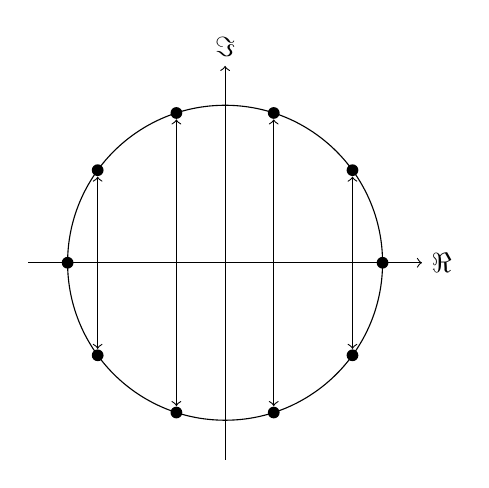
\begin{tikzpicture}[x=2cm,y=2cm] \draw (0,0) circle (1);

    \foreach \i in {0, ..., 9}
    \draw ({cos(\i*360/10)},{sin(\i*360/10)}) node[circle,fill,inner sep=1.5pt] (m\i) {};

    \draw[<->] (m1) -- (m9);
    \draw[<->] (m2) -- (m8);
    \draw[<->] (m3) -- (m7);
    \draw[<->] (m4) -- (m6);

    \draw[->] (-1.25,0) -- (+1.25,0) node[right] {$\Re$};
    \draw[->] (0,-1.25) -- (0,+1.25) node[above] {$\Im$};
  \end{tikzpicture}

  The action of $G_\RR$ on $\mu_{10} (\CC)$.
\end{center}

As an abelian group, $\mu_m (\CC)$ is non-canonically isomorphic to
$\ZZ/m\ZZ$. Similarly, the group of all roots of unity
$\colim_m \mu_m (\CC) = \bigoplus_p \dirlim_r \mu_{p^r} (\CC)$ is isomorphic to
$\QQ/\ZZ \isom \bigoplus_p \QQ_p/\ZZ_p$. Now we are going to write down such
isomorphisms in a canonical way, without forgetting about the action of
$G_\RR$. Further, we introduce a twist by $n$. In the setting of this text, $n$
is a negative integer, but for the sake of completeness, let us do that for any
integer $n$.

\begin{definition}[Tate twists]
  Let $n \in \ZZ$.

  \begin{itemize}
  \item If $n = 0$, then
    $$\mu_m (\CC)^{\otimes 0} \dfn \ZZ/m\ZZ,$$
    where $\ZZ/m\ZZ$ is taken with the trivial action of $G_\RR$.

  \item If $n > 0$, then
    \[ \mu_m (\CC)^{\otimes n} \dfn
      \underbrace{\mu_m (\CC)\otimes\cdots\otimes\mu_m (\CC)}_n \]
    is the $n$-th tensor power of $\mu_m (\CC)$ with the canonical action of
    $G_\RR$.

  \item If $n < 0$, then
    \[ \mu_m (\CC)^{\otimes n} \dfn
      \iHom (\mu_m (\CC)^{\otimes (-n)}, \ZZ/m\ZZ), \]
    where in this case the action of $G_\RR$ is given by
    $$\overline{f} (z) \dfn f (\overline{z}).$$
  \end{itemize}
\end{definition}

\begin{lemma}
  There is a canonical isomorphism of $G_\RR$-modules
  \begin{align*}
    \mu_m (\CC) & \xrightarrow{\isom} \frac{2\pi i \, \ZZ}{m\,(2\pi i)\,\ZZ},\\
    e^{2\pi i k/m} & \mapsto 2\pi i k.
  \end{align*}

  \begin{proof}
    The given explicit map is pretty self-explanatory, but the reader might
    appreciate the fact that this comes from the snake lemma. Let us consider
    the following morphism of short exact sequences of $G_\RR$-modules:

    \[ \begin{tikzcd}
        0 \ar{r} & 2\pi i \, \ZZ \ar{r}\ar{d}{-\times m} & \CC \ar{r}{z\mapsto e^z}\ar{d}{-\times m} & \CC^\times \ar{r}\ar{d}{(-)^m} & 1 \\
        0 \ar{r} & 2\pi i \, \ZZ \ar{r} & \CC \ar{r}{z\mapsto e^z} & \CC^\times \ar{r} & 1
      \end{tikzcd} \]

    Note that all the involved arrows are $G_\RR$-equivariant. The map in the
    middle has trivial kernel and cokernel, so by the snake lemma, there is a
    canonical isomorphism between the kernel of the last map, which is
    $\mu_m (\CC)$, and the cokernel of the first map, which is
    $\frac{2\pi i \, \ZZ}{m \, (2\pi i)\,\ZZ}$:
    $$\mu_m (\CC) \xrightarrow{\isom} \frac{2\pi i \, \ZZ}{m \, (2\pi i)\,\ZZ}.$$

    \[ \begin{tikzpicture}
        \matrix(m)[matrix of math nodes, row sep=3em, column sep=3em, text height=1.5ex, text depth=0.25ex]{
          0 & 0 & 0 & \mu_m (\CC) & ~ \\
          0 & 2\pi i\,\ZZ & \CC & \CC^\times & 1 \\
          0 & 2\pi i\,\ZZ & \CC & \CC^\times & 1 \\
          ~ & \frac{2\pi i\,\ZZ}{m\,(2\pi i)\,\ZZ} & 0 & 1 & 1\\};

        \path[->] (m-1-1) edge (m-1-2);
        \path[->] (m-1-2) edge (m-1-3);
        \path[->] (m-1-3) edge (m-1-4);

        \path[->] (m-2-1) edge (m-2-2);
        \path[->] (m-2-2) edge (m-2-3);
        \path[->,font=\scriptsize] (m-2-3) edge node[above] {$z\mapsto e^z$} (m-2-4);
        \path[->] (m-2-4) edge (m-2-5);

        \path[->] (m-3-1) edge (m-3-2);
        \path[->] (m-3-2) edge (m-3-3);
        \path[->,font=\scriptsize] (m-3-3) edge node[above] {$z\mapsto e^z$} (m-3-4);
        \path[->] (m-3-4) edge (m-3-5);

        \path[->] (m-4-2) edge (m-4-3);
        \path[->] (m-4-3) edge (m-4-4);
        \path[->] (m-4-4) edge (m-4-5);

        \path[>->] (m-1-2) edge (m-2-2);
        \path[>->] (m-1-3) edge (m-2-3);
        \path[>->] (m-1-4) edge (m-2-4);

        \path[->,font=\scriptsize] (m-2-2) edge node[pos=0.3,right] {$-\times m$} (m-3-2);
        \path[->,font=\scriptsize] (m-2-3) edge node[pos=0.3,right] {$-\times m$} (m-3-3);
        \path[->,font=\scriptsize] (m-2-4) edge node[pos=0.3,right] {$(-)^m$} (m-3-4);

        \path[->>] (m-3-2) edge (m-4-2);
        \path[->>] (m-3-3) edge (m-4-3);
        \path[->>] (m-3-4) edge (m-4-4);

        \draw[->,rounded corners] (m-1-4)
        to ($(m-1-4)!.6!(m-1-5)$)
        to ($(m-2-4)!.6!(m-2-5)$)
        to ($.2*(m-2-4)+.3*(m-2-5)+.2*(m-3-4)+.3*(m-3-5)$)
        to ($(m-2-4)!.5!(m-3-4)$)
        to ($(m-2-2)!.5!(m-3-2)$)
        to ($.3*(m-2-1)+.2*(m-2-2)+.3*(m-3-1)+.2*(m-3-2)$)
        to ($(m-3-1)!.4!(m-3-2)$)
        to ($(m-4-1)!.4!(m-4-2)$)
        to (m-4-2);
      \end{tikzpicture} \]
  \end{proof}
\end{lemma}

\begin{lemma}
  For $n > 0$ we have a canonical isomorphism of $G_\RR$-modules
  $$\mu_m (\CC)^{\otimes n} \isom \frac{(2\pi i)^n}{m\,(2\pi i)^n\,\ZZ}.$$

  \begin{proof}
    From the previous calculation and the canonical $G_\RR$-equivariant
    isomorphism
    \begin{align*}
      \underbrace{(2\pi i)\,\ZZ\otimes\cdots\otimes (2\pi i)\,\ZZ}_n & \xrightarrow{\isom} (2\pi i)^n\,\ZZ, \\
      (2\pi i)\,a_1\otimes\cdots\otimes (2\pi i)\,a_n & \mapsto (2\pi i)^n\,a_1\cdots a_n
    \end{align*}
    we obtain
    \[ \underbrace{\mu_m (\CC)\otimes\cdots\otimes\mu_m (\CC)}_n \xrightarrow{\isom}
      \underbrace{\frac{2\pi i \, \ZZ}{m \, (2\pi i)\,\ZZ}\otimes\cdots\otimes\frac{2\pi i \, \ZZ}{m \, (2\pi i)\,\ZZ}}_n \isom
      \frac{(2\pi i)^n\,\ZZ}{m \, (2\pi i)^n\,\ZZ}. \]
  \end{proof}
\end{lemma}

\begin{lemma}
  \label{lemma:roots-of-unity-GR-equiv}
  For $n < 0$ we have a canonical isomorphism of $G_\RR$-modules
  \[ \mu_m (\CC)^{\otimes n} \dfn
    \iHom (\mu_m^{\otimes (-n)} (\CC), \ZZ/m\ZZ) \isom
    \frac{(2\pi i)^n \, \ZZ}{m \, (2\pi i)^n \, \ZZ}. \]

  \begin{proof}
    We claim that there is a $G_\RR$-equivariant isomorphism
    \begin{equation}
      \label{eqn:dual-conjugation}
      \iHom \left(\frac{(2\pi i)^{-n}\,\ZZ}{m \, (2\pi i)^{-n}\,\ZZ}, \ZZ/m \ZZ\right) \isom
      \iHom \left((2\pi i)^{-n}\,\ZZ, ~ \ZZ/m \ZZ\right) \xrightarrow{\isom}
      \frac{(2\pi i)^n\,\ZZ}{m \, (2\pi i)^n\,\ZZ}.
    \end{equation}

    Note that $-n$ got replaced with $n$, for the reason which will be apparent
    in a second. A homomorphism $f\colon (2\pi i)^{-n}\,\ZZ \to \ZZ/m \ZZ$ is
    determined by the image of a generator $f ((2\pi i)^{-n}\cdot 1)$, so we may
    define the second isomorphism in \eqnref{eqn:dual-conjugation} by
    \begin{equation}
      \label{eqn:dual-conjugation-dfn}
      \Phi\colon f \mapsto (2\pi i)^n \cdot f ((2\pi i)^{-n}\cdot 1).
    \end{equation}

    It is clearly an isomorphism of abelian groups, and it only remains to check
    that it is $G_\RR$-equivariant, i.e. that for all
    $f\colon (2\pi i)^{-n}\,\ZZ \to \ZZ/m \ZZ$ holds
    $$\Phi (\overline{f}) = \overline{\Phi (f)}.$$
    We have indeed
    \begin{multline*} \Phi (\overline{f}) = (2\pi i)^n \cdot \overline{f} ((2\pi i)^{-n}\cdot 1) = (2\pi i)^n \cdot f (\overline{(2\pi i)^{-n}\cdot 1}) \\
      = (-1)^n \, (2\pi i)^n \cdot f ((2\pi i)^{-n}\cdot 1)
    \end{multline*}
    and
    \[ \overline{\Phi (f)} =
      \overline{(2\pi i)^n \cdot f ((2\pi i)^{-n}\cdot 1)} =
      (-1)^n \, (2\pi i)^n \cdot f ((2\pi i)^{-n}\cdot 1). \]
  \end{proof}
\end{lemma}

\begin{lemma}
  \label{lemma:all-roots-of-unity-as-QZ}
  The $G_\RR$-module of all roots of unity twisted by $n$ is canonically
  isomorphic to the $G_\RR$-module $\frac{(2\pi i)^n\,\QQ}{(2\pi i)^n\,\ZZ}$:
  \[ \colim_m \mu_m (\CC)^{\otimes n} \dfn
    \bigoplus_p \dirlim_r \mu_{p^r} (\CC)^{\otimes n} \isom
    \frac{(2\pi i)^n\,\QQ}{(2\pi i)^n\,\ZZ}. \]

  \begin{proof}
    Using the previous calculations and observing that the transition morphisms
    in the colimit are $G_\RR$-equivariant,
    \[ \bigoplus_p \dirlim_r \mu_{p^r} (\CC)^{\otimes n} \isom
      \bigoplus_p \dirlim_r \frac{(2\pi i)^n\,\ZZ}{p^r\,(2\pi i)^n\,\ZZ} \isom
      \frac{(2\pi i)^n\,\QQ}{(2\pi i)^n\,\ZZ}. \]
  \end{proof}
\end{lemma}

Somewhat abusively, from now on we will write simply ``$(2\pi i)^n\,\QQ/\ZZ$''
for $\frac{(2\pi i)^n\,\QQ}{(2\pi i)^n\,\ZZ}$.

% % % % % % % % % % % % % % % % % % % % % % % % % % % % % % 

\section{$G$-equivariant sheaves}
\label{section:equivariant-sheaves}

$G$-equivariant sheaves on topological spaces are discussed in Grothendieck's
Tohoku paper \cite{Tohoku-paper}:

\begin{quote}
  Nous appelerons $G$-faisceau sur $X = X(G)$ un faisceau (d'ensembles) $A$
  sur $X$, dans lequel $G$ opère de façon compatible avec ses opérations
  sur $X$. Pour donner un sens à cette définition, on pourra par exemple
  considérer $A$ comme espace étalé dans $X$; nous n'insisterons pas.
\end{quote}

In this section I will give some explanation of the notion of a $G$-equivariant
sheaf and collect certain relevant results. What follows is a rather
straightforward generalization of the usual sheaf theory, so I omit some
details. Probably the best way to motivate the definition is to recall the
construction of the sheaf of sections of a continuous map.

\begin{nameless}\textbf{Classical example.}
  Let $X$ be a topological space. Consider the category $\categ{Top}_{/X}$ of
  spaces over $X$ where the objects are continuous maps of topological spaces
  $p\colon E\to X$ and the morphisms are commutative diagrams
  \begin{equation}
    \label{eqn:morphism-of-spaces-over-X}
    \begin{tikzcd}[row sep=small, column sep=small]
      E\ar{rr}{f}\ar{dr}[swap]{p} && E'\ar{dl}{p'} \\
      & X
    \end{tikzcd}
  \end{equation}

  For a topological space over $X$ given by $p\colon E\to X$, the corresponding
  \term{sheaf of sections} is the sheaf of sets defined by
  \[ \mathcal{F} (U) \dfn \Hom_{\categ{Top}_{/X}} (U, E) =
    \left\{ \begin{tikzcd}[row sep=small, column sep=small]
        U \ar{rr}{s}\ar[hookrightarrow]{dr} & & E\ar{dl}{p} \\
        & X
      \end{tikzcd} \right\} \]
  for each open subset $U \subset X$. The restriction maps are obvious:
  an inclusion of open subsets $i\colon V \hookrightarrow U$ induces
  contravariantly
  \[ \res_{VU} \dfn \Hom_{\categ{Top}_{/X}} (i, E)\colon
    \mathcal{F} (U) \to \mathcal{F} (V), \]
  and the sheaf axiom is also easy to verify. A morphism over $X$ of the form
  \eqnref{eqn:morphism-of-spaces-over-X} gives rise to a morphism of the
  corresponding sheaves of sections: for each open subset $U \subset X$ we get a
  map
  \begin{align*}
    \phi_U\colon \Hom_{\categ{Top}_{/X}} (U, E) & \to \Hom_{\categ{Top}_{/X}} (U, E'),\\
    \begin{tikzcd}[row sep=small, column sep=small,ampersand replacement=\&] U
      \ar{rr}{s}\ar[hookrightarrow]{dr} \&\& E\ar{dl}{p} \\
      \& X
    \end{tikzcd} & \mapsto \begin{tikzcd}[row sep=small, column sep=small,ampersand replacement=\&]
      U \ar{r}{s}\ar[hookrightarrow]{dr} \& E\ar{d}{p}\ar{r}{f} \& E'\ar{dl}{p'} \\
      \& X
    \end{tikzcd}
  \end{align*}
  and for each $V\subset U$ the diagram
  \[ \begin{tikzcd}
      \mathcal{F} (U) \dfn \Hom_{\categ{Top}_{/X}} (U, E)\ar{r}{\phi_U}\ar{d}[swap]{\res_{VU}} & \Hom_{\categ{Top}_{/X}} (U, E')\ar{d}{\res_{VU}'} \rdfn \mathcal{F}' (U) \\
      \mathcal{F} (V) \dfn \Hom_{\categ{Top}_{/X}} (V, E)\ar{r}{\phi_V} & \Hom_{\categ{Top}_{/X}} (V, E') \rdfn \mathcal{F}' (V)
    \end{tikzcd} \]
  clearly commutes. So formation of the sheaf of sections is a functor
  $$\Gamma\colon \categ{Top}_{/X} \to \categ{Sh} (X).$$
\end{nameless}

\begin{nameless}\textbf{$G$-equivariant example.}
  \label{obs:G-equivariant-sheaf-of-sections}
  For a discrete group $G$, consider the category of $G$-spaces $G\categ{-Top}$
  where the objects are topological spaces $X$ with a specified action of $G$ by
  homeomorphisms $\sigma_X\colon G\times X\to X$, and morphisms $f\colon X\to Y$
  are continuous $G$-equivariant maps:

  \[ \begin{tikzcd}
      G\times X\ar{r}{\idid\times f}\ar{d}[swap]{\sigma_X} & G\times Y\ar{d}{\sigma_Y} \\
      X\ar{r}{f} & Y
    \end{tikzcd} \]

  For a fixed $G$-space $X$, the category $G\categ{-Top}_{/X}$ of
  \term{$G$-spaces over $X$} has as its objects continuous $G$-equivariant maps
  $p\colon E\to X$ and as morphisms continuous $G$-equivariant maps over $X$
  \[ \begin{tikzcd}[row sep=small, column sep=small]
      E\ar{rr}{f}\ar{dr}[swap]{p} && E'\ar{dl}{p'} \\
      & X
    \end{tikzcd} \]
  For a $G$-space over $X$ given by $p\colon E\to X$, the corresponding sheaf of
  sections $\mathcal{F}$ carries the following extra datum. For each open subset
  $U \subset X$ and each $g\in G$ there is a bijection of sets
  \begin{align*}
    \alpha_{g,U}\colon \mathcal{F} (U) & \xrightarrow{\isom} \mathcal{F} (g\cdot U), \\
    (s\colon U\to E) & \mapsto \left(\begin{array}{rcl}
                                       g\cdot U & \to & E,\\
                                       g\cdot u & \mapsto & g\cdot s (u)
                                     \end{array}\right),\\
    \left(\begin{array}{rcl}
            U & \to & E, \\
            u & \mapsto & g^{-1}\cdot s (g\cdot u)
          \end{array}\right) & \mapsfrom (s\colon g\cdot U\to E).
  \end{align*}

  Using the fact that $p$ is $G$-equivariant, one checks that $\alpha_{g,U}$
  indeed sends sections over $U$ to sections over $g\cdot U$. We also see that
  the bijections $\alpha_{g,U}$ satisfy the following properties:

  \begin{enumerate}
  \item[1)] compatibility with restrictions: for open subsets $V\subset U$ the
    diagram
    \[ \begin{tikzcd}
        \mathcal{F} (U)\ar{r}{\alpha_{g,U}}[swap]{\isom}\ar{d}[swap]{\res_{VU}} & \mathcal{F} (g\cdot U)\ar{d}{\res_{g\cdot V,g\cdot U}} \\
        \mathcal{F} (V)\ar{r}{\alpha_{g,V}}[swap]{\isom} & \mathcal{F} (g\cdot V)
      \end{tikzcd} \]
    commutes;

  \item[2)] for the identity element $1\in G$ and each open subset $U \subset X$
    we have
    $$\alpha_{1,U} = \idid\colon \mathcal{F} (U) \to \mathcal{F} (U);$$

  \item[3)] the cocycle condition: for each open subset $U \subset X$ and
    $g,h\in G$ the diagram
    \[ \begin{tikzcd}[row sep=small, column sep=small]
        & \mathcal{F} (h\cdot U) \ar{dr}{\alpha_{g,h\cdot U}} \\
        \mathcal{F} (U)\ar{ur}{\alpha_{h,U}}\ar{rr}[swap]{\alpha_{gh,U}} & & \mathcal{F} (gh\cdot U)
      \end{tikzcd} \]
  commutes.
  \end{enumerate}

  For a morphism of $G$-spaces over $X$
  \[ \begin{tikzcd}[row sep=small, column sep=small]
      E\ar{rr}{f}\ar{dr}[swap]{p} && E'\ar{dl}{p'} \\
      & X
    \end{tikzcd} \]
  the corresponding morphism of sheaves of sections
  $\phi\colon \mathcal{F} \to \mathcal{F}'$ is easily seen to be compatible with
  the maps $\alpha_{g,U}$ and $\alpha_{g,U}'$: for each $U \subset X$ the
  diagram
  \[ \begin{tikzcd}
      \mathcal{F} (U) \ar{r}{\phi_U}\ar{d}[swap]{\alpha_{g,U}} & \mathcal{F}' (U) \ar{d}{\alpha'_{g,U}} \\
      \mathcal{F} (g\cdot U) \ar{r}{\phi_{g\cdot U}} & \mathcal{F}' (g\cdot U)
    \end{tikzcd} \]
  commutes.
\end{nameless}

Now hopefully, the last example makes the following definition look natural.

\begin{definition}
  \label{dfn:equivariant-sheaves}
  Let $G$ be a discrete group and let $X$ be a $G$-space. Then a
  \term{$G$-equivariant presheaf} (of sets) on $X$ is a presheaf $\mathcal{F}$
  equipped with bijections of sets
  $$\alpha_{g,U}\colon \mathcal{F} (U) \xrightarrow{\isom} \mathcal{F} (g\cdot U)$$
  for each $g\in G$ and open subset $U\subset X$ that satisfy the following
  axioms:

  \begin{enumerate}
  \item[1)] these bijections are compatible with restrictions:

    \[ \begin{tikzcd}
      \mathcal{F} (U)\ar{r}{\alpha_{g,U}}[swap]{\isom}\ar{d}[swap]{\res_{VU}} & \mathcal{F} (g\cdot U)\ar{d}{\res_{g\cdot V,g\cdot U}} \\
      \mathcal{F} (V)\ar{r}{\alpha_{g,V}}[swap]{\isom} & \mathcal{F} (g\cdot V)
    \end{tikzcd} \]

  \item[2)] $\alpha_{1,U} = \idid\colon \mathcal{F} (U) \to \mathcal{F} (U)$;

  \item[3)] for $g,h\in G$ the cocycle condition holds:
    \[ \begin{tikzcd}[row sep=small, column sep=small]
        & \mathcal{F} (h\cdot U) \ar{dr}{\alpha_{g,h\cdot U}} \\
        \mathcal{F} (U)\ar{ur}{\alpha_{h,U}}\ar{rr}[swap]{\alpha_{gh,U}} & & \mathcal{F} (gh\cdot U)
    \end{tikzcd} \]
  \end{enumerate}

  A \term{$G$-equivariant sheaf} is a $G$-equivariant presheaf satisfying the
  usual sheaf axiom: for each open covering $U = \bigcup_i U_i$ we have an
  equalizer
  \[ \mathcal{F} (U) \to \prod_i \mathcal{F} (U_i) \rightrightarrows
    \prod_{i,j} \mathcal{F} (U_i\cap U_j). \]

  A \term{morphism of $G$-equivariant (pre)sheaves}
  $\mathcal{F} \to \mathcal{F}'$ is a morphism of (pre)sheaves which is
  compatible with the maps $\alpha_{g,U}$:
  \[ \begin{tikzcd}
      \mathcal{F} (U) \ar{r}{\phi_U}\ar{d}[swap]{\alpha_{g,U}} & \mathcal{F}' (U) \ar{d}{\alpha'_{g,U}} \\
      \mathcal{F} (g\cdot U) \ar{r}{\phi_{g\cdot U}} & \mathcal{F}' (g\cdot U) \\
    \end{tikzcd} \]

  We denote the category of $G$-equivariant presheaves (resp. sheaves) on $X$ by
  $\categ{PSh} (G,X)$ (resp. $\categ{Sh} (G,X)$).
\end{definition}

We may summarize \ref{obs:G-equivariant-sheaf-of-sections} by saying that taking
the sheaf of sections is a functor
$$\Gamma\colon G\categ{-Top}_{/X} \to \categ{Sh} (G,X).$$
It commutes with the forgetful functors:
\[ \begin{tikzcd}
    G\categ{-Top}_{/X} \ar{r}{\Gamma}\ar{d} & \categ{Sh} (G,X)\ar{d} \\
    \categ{Top}_{/X} \ar{r}{\Gamma} & \categ{Sh} (X)
  \end{tikzcd} \]

\begin{remark}
  Despite the extra datum coming from the action of $G$, the category
  $\categ{Sh} (G,X)$ is still a Grothendieck topos. This can be deduced from
  Giraud's characterization of Grothendieck toposes \cite[Exposé~IV, 1.2]{SGA4}
  (see e.g. \cite[Appendix]{MacLane-Moerdijk-94} for details). However, the
  underlying Grothendieck site is not obvious.
\end{remark}

\begin{observation}
  The global sections $\mathcal{F} (X)$ of a $G$-equivariant (pre)sheaf is a
  $G$-set with the action of $G$ given by
  \[ \alpha_{g,X}\colon \mathcal{F} (X) \xrightarrow{\isom}
    \mathcal{F} (g\cdot X) = \mathcal{F} (X). \]
  Taking the global sections is a functor
  $$\categ{PSh} (G,X) \to G\categ{-Set}.$$

  \begin{proof}
    The axioms $\alpha_{1,X} = \idid$ and
    $\alpha_{gh,X} = \alpha_{g,h\cdot X}\circ \alpha_{h,X}$ correspond to the
    axioms of a group action.
  \end{proof}
\end{observation}

\begin{example}
  Let $\mathcal{F}$ be the sheaf of sections of a $G$-space over $X$ given by
  $p\colon E\to X$. Then the action of $g\in G$ on $\mathcal{F} (X)$ sends a
  global section $s\colon X\to E$ to the global section
  \begin{align*}
    X & \to E, \\
    x & \mapsto g\cdot s (g^{-1}\cdot x).
  \end{align*}
  (see the formula for $\alpha_{g,U}$ in
  \ref{obs:G-equivariant-sheaf-of-sections}).
\end{example}

\begin{definition}
  \label{def:constant-G-equivariant-presheaf}
  Let $S$ be a $G$-set. For a $G$-space $X$, consider the presheaf $S_X$ defined
  by $S_X (U) = S$ for each open subset $U \subset X$ with the identity
  restriction maps. The morphisms
  \begin{align*}
    \alpha_{g,U} = \sigma_g\colon S_X (U) & \to S_X (g\cdot U),\\
    x & \mapsto g\cdot x.
  \end{align*}
  define a structure of a $G$-equivariant presheaf on $S_X$, called the
  \term{constant $G$-equivariant presheaf} associated to $S$.
\end{definition}

\begin{observation}
  Formation of the constant $G$-equivariant presheaf is a functor
  $$G\categ{-Set} \to \categ{PSh} (G,X),$$
  which is left adjoint to the global section functor:
  \[ \Hom_{\categ{PSh} (G,X)} (S_X, \mathcal{P}) \isom
    \Hom_{G\categ{-Set}} (S, \mathcal{P} (X)). \]

  \begin{proof}
    A morphism of $G$-equivariant presheaves $S_X \to \mathcal{P}$ is given by a
    collection of maps $\phi_U\colon S \to \mathcal{P} (U)$ that are compatible
    with the restriction maps and the $G$-equivariant structure morphisms:

    \[ \begin{tikzcd}
        S\ar{r}{\phi_X}\ar{dr}{\phi_U}\ar{ddr}[swap]{\phi_V} & \mathcal{P} (X)\ar[bend left=60]{dd}{\res_{VX}}\ar{d}{\res_{UX}} && S\ar{d}[swap]{\sigma_g}\ar{r}{\phi_U} & \mathcal{P} (U) \ar{d}{\alpha_{g,U}} \\
        & \mathcal{P} (U)\ar{d}{\res_{VU}} && S\ar{r}{\phi_{g\cdot U}} & \mathcal{P} (g\cdot U) \\ & \mathcal{P} (V)
      \end{tikzcd} \]

    From the first diagram we see that $\phi_U = \res_{UX}\circ\phi_X$, so that
    the map $\phi_X\colon S\to \mathcal{P} (X)$ defines the rest, and from the
    second diagram we see that it is $G$-equivariant. This shows that the
    bijection in question is given by
    \begin{align*}
      \{ \phi_U \} & \mapsto \phi_X,\\
      \{ \phi_U \dfn \res_{UX}\circ\phi \} & \mapsfrom \phi.
    \end{align*}
  \end{proof}
\end{observation}

\subsection*{Alternative definition via $G$-equivariant espaces étalés}

One says that a continuous map $p\colon E\to X$ is \term{étale}\footnote{This is
  in fact the topological counterpart of étale morphisms of schemes.} if it is a
local on the source homeomorphism (for each $e\in E$ there exists an open
neighborhood $V\ni p$ such that $p (V)$ is open in $X$ and
$\left.p\right|_V\colon V \to p (V)$ is a homeomorphism). We have a full
subcategory
$$G\categ{-Ét}_{/X} \subset G\categ{-Top}_{/X}$$
formed by $G$-spaces that are étale over $X$. We note that if $p$ and $p'$ are
étale and we have a commutative diagram
\[ \begin{tikzcd}[row sep=small, column sep=small]
    E\ar{rr}{f}\ar{dr}[swap]{p} && E'\ar{dl}{p'} \\
    & X
\end{tikzcd} \]
then $f$ is étale as well, so that the morphisms in $G\categ{-Ét}_{/X}$ are
automatically étale. The importance of étale spaces over $X$ is explained by the
following well-known result, which we state $G$-equivariantly.

\begin{proposition}
  Let $\mathcal{F}$ be a $G$-equivariant presheaf on $X$. Consider the disjoint
  union of stalks
  \[ \coprod_{x\in X} \mathcal{F}_x, \quad
    \mathcal{F}_x \dfn \dirlim_{U\ni x} \mathcal{F} (U). \]
  It carries a natural action of $G$. For each section $s\in \mathcal{F} (U)$
  such that $U\ni x$, denote by $s_x \in \mathcal{F}_x$ the corresponding germ
  at $x$. This defines a map between sets (which we again denote by $s$)
  \begin{align*}
    s\colon U & \to \coprod_{x\in X} \mathcal{F}_x,\\
    x & \mapsto s_x.
  \end{align*}

  Consider now the topology on $\coprod_{x\in X} \mathcal{F}_x$ generated by
  $s (U)$ for all open subsets $U \subset X$ and all
  $s\in \mathcal{F} (U)$. Then the action of $G$ is continuous with respect to
  this topology, and the natural projection
  \begin{align*}
    p\colon \coprod_{x\in X} \mathcal{F}_x & \to X,\\
    \mathcal{F}_x \ni s_x & \mapsto x.
  \end{align*}
  is an étale $G$-equivariant map.

  \begin{proof} This is a well-known, basic result
    (see e.g. \cite[Chapter~II]{MacLane-Moerdijk-94}); one just has to check the
    $G$-equivariance.
  \end{proof}
\end{proposition}

This leads to an equivalent definition of $G$-equivariant sheaves.

\begin{nameless}\textbf{Alternative definition.}
  Let $G$ be a group and $X$ be a $G$-space. Then a \term{$G$-equivariant sheaf}
  on $X$ is an étale $G$-space over $X$
  $$p\colon E\to X,$$
  and a morphism of $G$-equivariant sheaves is a morphism over $X$
  \[ \begin{tikzcd}[row sep=small, column sep=small]
      E\ar{rr}{f}\ar{dr}[swap]{p} && E'\ar{dl}{p'} \\
      & X
    \end{tikzcd} \]
\end{nameless}

\begin{remark}
  Note that the above definition looks more natural than
  \ref{dfn:equivariant-sheaves}. It also generalizes to the case a topological
  group $G$ acting on $E$ and $X$ continuously. This is not possible in
  \ref{dfn:equivariant-sheaves}, because there we consider only how each
  separate element $g\in G$ acts on $X$.
\end{remark}

\begin{example}
  \label{example:constant-G-equivariant-sheaf-as-esace-etale}
  In these terms, it is easier to describe equivariant sheafification and what a
  constant sheaf is. If $S$ is a $G$-set and $X$ is a $G$-space, we may endow
  $S$ with the discrete topology and consider the $G$-space $S\times X$ with the
  component-wise action of $G$ (which is the product in the category of
  $G$-spaces). Then the projection $S\times X\to X$ is an étale $G$-equivariant
  map, so it corresponds to some $G$-equivariant sheaf. We call it the
  \term{constant $G$-equivariant sheaf} associated to $S$. This construction is
  obviously functorial: a $G$-equivariant map $S \to S'$ induces a morphism in
  $G\categ{-Ét}_{/X}$
  \[ \begin{tikzcd}[row sep=small, column sep=small]
      S\times X\ar{rr}\ar{dr} & & S'\times X\ar{dl} \\
      & X
  \end{tikzcd} \]
\end{example}

\subsection*{Abelian $G$-equivariant sheaves and their cohomology}

\begin{proposition}
  Let $X$ be a $G$-space. Consider the category $\categ{Sh} (G,X)^\categ{Ab}$ of
  $G$-equivariant sheaves of abelian groups on $X$ (defined, for instance, as
  abelian group objects in the category of $G$-equivariant sheaves of sets).
  It is an abelian category with enough injectives.

  \begin{proof}
    The usual argument of Grothendieck works: any abelian category which
    satisfies the axiom AB5) and has generators has enough injectives
    \cite[Ch.~I, 1.10]{Tohoku-paper}. This is the case for
    $\categ{Sh} (G,X)^\categ{Ab}$ (as for the generators, see
    \cite[Appendix]{MacLane-Moerdijk-94}).
  \end{proof}
\end{proposition}

\begin{example}
  Let $A$ be a $G$-set (resp. $G$-module). Then the associated constant sheaf
  $\underline{A}$ has a canonical $G$-equivariant abelian sheaf structure.
\end{example}

\begin{example}
  Consider some topological space with an action of the Galois group
  $G_\RR \dfn \Gal (\CC/\RR)$; for instance, the set of complex points of
  a scheme $X (\CC)$ equipped with the analytic topology. Then the complex
  $m$-th roots of unity $\mu_m (\CC)$ (reviewed above in
  \S\ref{section:roots-of-unity}) give us a constant $G_\RR$-equivariant sheaf
  on $X (\CC)$. This is the only example we will be interested in.
\end{example}

\begin{definition}
  The equivariant global section functor
  \begin{align*}
    \Gamma (G,X,-)\colon \categ{Sh} (G,X)^\categ{Ab} & \to \categ{Ab},\\
    \mathcal{F} & \rightsquigarrow \mathcal{F} (X)^G
  \end{align*}
  is left exact. Here the global sections
  \[ \mathcal{F} (X) \dfn
    \{ s\colon X\to \Et (\mathcal{F}) \mid \pi\circ s = \id{X} \} \]
  come with an action of $G$ by
  $$(g\cdot s) (x) \dfn g\cdot s (g^{-1}\cdot x).$$
  (Note that in general, $\mathcal{F} (U)$ carries such an action of $G$,
  whenever $U \subset X$ is closed under the action of $G$.) The fixed points of
  this action are precisely the $G$-equivariant sections, i.e. sections that
  satisfy $s (g\cdot x) = g\cdot (s (x))$. The right derived functors of
  $\Gamma (G,X,-)$ are by definition $R\Gamma (G, X, \mathcal{F})$.
\end{definition}

This is related to the usual sheaf cohomology by
\begin{equation}
  \label{eqn:grothendieck-ss-for-equivariant-sheaves}
  R\Gamma (G, X, \mathcal{F}) \isom R\Gamma (G, R\Gamma (X, \mathcal{F})),
\end{equation}
where the right hand side is the group cohomology. Indeed, $\Gamma (G,X,-)$ is a
composition of two left exact functors: the usual global section functor and the
fixed points functor
\[ \categ{Sh} (G,X)^\categ{Ab}
  \xrightarrow{\mathcal{F} \rightsquigarrow \mathcal{F} (X)}
  G\categ{-Mod} \xrightarrow{A \rightsquigarrow A^G} \categ{Ab} \]
and \eqnref{eqn:grothendieck-ss-for-equivariant-sheaves} are the derived
functors of a composition of functors (this is known as the
\term{Grothendieck spectral sequence}; see e.g. \cite[\S 10.8]{Weibel-94}). On
the level of cohomology, we have a spectral sequence
\[ E_2^{pq} = H^p (G, H^q (X,\mathcal{F})) \Longrightarrow
  H^{p+q} (G,X,\mathcal{F}). \]

% % % % % % % % % % % % % % % % % % % % % % % % % % % % % %

\section{From étale to analytic sheaves
  \mbox{(the morphism \texorpdfstring{$\alpha^*$}{α\^{}∗})}}
\label{section:etale-and-equivariant-sheaves}

The canonical reference for comparison between étale and singular cohomology is
\cite[Exposé~XI, \S 4]{SGA4}, so let us to borrow some definitions and notation
from there. Let $X$ be an arithmetic scheme (separated, of finite type over
$\Spec \ZZ$).

\begin{enumerate}
\item The base change from $\Spec \ZZ$ to $\Spec \CC$
  \[ \begin{tikzpicture}
      \matrix(m)[matrix of math nodes, row sep=2em, column sep=2em, text height=1.5ex, text depth=0.25ex]{
        X_\CC & X \\
        \Spec \CC & \Spec \ZZ\\};
      \path[->] (m-1-1) edge (m-1-2);
      \path[->] (m-1-1) edge (m-2-1);
      \path[->] (m-1-2) edge (m-2-2);
      \path[->] (m-2-1) edge (m-2-2);
      \begin{scope}[shift=($(m-1-1)!.4!(m-2-2)$)]
        \draw +(-.2,0) -- +(0,0) -- +(0,.2);
      \end{scope}
    \end{tikzpicture} \]
  gives us a morphism of sites
  $$\gamma\colon X_{\CC,\text{\it ét}} \to X_\text{\it ét}.$$

\item We denote by $X (\CC)$ the set of complex points of $X$ equipped with the
  usual analytic topology.

  Let $X_\text{\it cl}$ be the site of étale maps $f\colon U\to X (\CC)$.
  A covering family in $X_\text{\it cl}$ is a family of maps $\{ U_i \to U \}$
  such that $U$ is the union of images of $U_i$. The notation ``cl'' comes from
  SGA 4 and stays for ``classique''.

  As the inclusion of an open subset $U \subset X (\CC)$ is trivially an étale
  map, we have a fully faithful functor $X (\CC) \subset X_\text{\it cl}$, and
  the topology on $X (\CC)$ is induced by the topology on
  $X_\text{\it cl}$. This gives us a morphism of sites
  $$\delta\colon X_\text{\it cl} \to X (\CC),$$
  which by the well-known ``comparison lemma''
  \cite[Exposé~III, Théorème~4.1]{SGA4} induces an equivalence of the
  corresponding categories of sheaves
  $$\delta_*\colon \categ{Sh} (X_\text{\it cl}) \to \categ{Sh} (X (\CC)).$$

\item A morphism of schemes $f\colon X'_\CC \to X_\CC$ over $\Spec \CC$ is étale
  if and only if $f (\CC)\colon X' (\CC) \to X (\CC)$ is étale in the
  topological sense \cite[Exposé XII, Proposition 3.1]{SGA1}, and therefore the
  functor $X'_\CC \rightsquigarrow X' (\CC)$ gives us a morphism of sites
  $$\epsilon\colon X_\text{\it cl} \to X_{\CC,\text{\it ét}}.$$
\end{enumerate}

We may now consider the composite functor

\[ \begin{tikzcd}
    \categ{Sh} (X_\text{\it ét}) \ar{r}{\gamma^*} &
    \categ{Sh} (X_{\CC,\text{\it ét}}) \ar{r}{\epsilon^*} &
    \categ{Sh} (X_\text{\it cl}) \ar{r}{\delta_*}[swap]{\cequiv} &
    \categ{Sh} (X (\CC))
  \end{tikzcd} \]

\noindent where $\gamma^*$ is given by the base change from $\Spec \ZZ$ to
$\Spec \CC$, the functor $\epsilon^*$ is the comparison, and $\delta_*$ is an
equivalence of categories. As we start from a scheme over $\Spec \ZZ$ and base
change to $\Spec \CC$, the resulting sheaf on $X (\CC)$ is in fact equivariant
with respect to the complex conjugation, and the above composition gives us an
``inverse image'' functor
$$\alpha^*\colon \categ{Sh} (X_\text{\it ét}) \to \categ{Sh} (G_\RR, X (\CC)).$$

% % % % % % % % % % % % % % % % % % % % % % % % % % % % % % 

\section{Cohomology with compact support on
  \texorpdfstring{$X_\text{\it ét}$}{X\_ét} and $X (\CC)$}
\label{section:cohomology-with-compact-support}

For any arithmetic scheme $f\colon X\to \Spec \ZZ$ (separated, of finite type)
there exists a \term{Nagata compactification} $f = g\circ j$ where $j$ is an
open immersion and $g$ is a proper morphism:
\[ \begin{tikzcd}
    X \ar[hookrightarrow]{rr}{j}\ar{dr}[swap]{f} & & \mathfrak{X} \ar{dl}{g} \\
    & \Spec \ZZ
  \end{tikzcd} \]

This is a result of Nagata, and a modern exposition (following Deligne) may be
found in \cite{Conrad-Deligne-Nagata,Conrad-Deligne-Nagata-erratum}. See also
\cite[Exposé XVII]{SGA4}.

\begin{definition}
  Let $X$ be an arithmetic scheme and let $\mathcal{F}^\bullet$ be a complex of
  abelian torsion sheaves on $X_\text{\it ét}$. Then we define the
  \term{cohomology of $\mathcal{F}^\bullet$ with compact support} via the
  complex
  \begin{equation}
    \label{eqn:RGammac-via-extension-by-zero}
    R\Gamma_c (X_\text{\it ét}, \mathcal{F}^\bullet) \dfn
    R\Gamma (\mathfrak{X}_\text{\it \'et}, j_! \mathcal{F}^\bullet).
  \end{equation}
\end{definition}

For torsion sheaves, this does not depend on the choice of
$j\colon X \hookrightarrow \mathfrak{X}$, but here we would like to fix this
choice to be able to compare $j$ with the corresponding morphism
$j (\CC)\colon X (\CC) \hookrightarrow \mathfrak{X} (\CC)$. Note that thanks to
the \term{Leray spectral sequence}
$R\Gamma (\mathfrak{X}_\text{\it ét}, -) \isom R\Gamma (\Spec \ZZ_\text{\it ét}, -)\circ R g_*$
(that is, the Grothendieck spectral sequence coming from
$\Gamma (\mathfrak{X}_\text{\it ét}, -) = \Gamma (\Spec \ZZ_\text{\it ét}, -) \circ g_*$),
we have
\begin{equation}
  \label{eqn:RGammac-via-derived-lower-shriek}
  R\Gamma_c (X_\text{\it ét}, \mathcal{F}^\bullet) \isom
  R\Gamma (\Spec \ZZ_\text{\it \'et}, R f_! \mathcal{F}^\bullet),
\end{equation}
where by definition
$$R f_! \mathcal{F}^\bullet \dfn R g_* j_! \mathcal{F}^\bullet$$
(this is just a piece of notation, standard and quite unfortunate;
``$R f_!$'' does not mean that we are deriving $f_!$).

The formulas \eqnref{eqn:RGammac-via-extension-by-zero} and
\eqnref{eqn:RGammac-via-derived-lower-shriek} give two equivalent
definitions. We are going to use \eqnref{eqn:RGammac-via-derived-lower-shriek}
in the next section to introduce a slightly different version of cohomology with
compact support, denoted by
$R\widehat{\Gamma}_c (X_\text{\it ét}, \mathcal{F}^\bullet)$, which is needed
for arithmetic duality theorems. In this section, we need to use
\eqnref{eqn:RGammac-via-extension-by-zero} to define cohomology with compact
support on $X (\CC)$, in a way that allows us to compare it with cohomology with
compact support on $X_\text{\it ét}$.

\begin{definition}
  If $j\colon X\hookrightarrow \mathfrak{X}$ is a Nagata compactification, then
  we have the corresponding open immersion
  $$j (\CC)\colon X (\CC) \to \mathfrak{X} (\CC),$$
  and for a sheaf $\mathcal{F}$ on $X (\CC)$ we define
  \[ \Gamma_c (X (\CC), \mathcal{F}) \dfn
    \Gamma (\mathfrak{X} (\CC), j (\CC)_! \mathcal{F}). \]
  Similarly, for a $G_\RR$-equivariant sheaf on $X (\CC)$ we define
  \[ \Gamma_c (G_\RR, X (\CC), \mathcal{F}) \dfn
    \Gamma (G_\RR, \mathfrak{X} (\CC), j (\CC)_! \mathcal{F}). \]
\end{definition}

\begin{proposition}
  \label{prop:inverse-image-gamma}
  Let $\mathcal{F}$ be a sheaf on $X_\text{\it ét}$.

  \begin{enumerate}
  \item[1)] There exists a morphism
    \[ \Gamma (X_\text{\it ét}, \mathcal{F}) \to
      \Gamma (G_\RR, X (\CC), \alpha^* \mathcal{F}), \]
    which is natural in the sense that every morphism of sheaves
    $\mathcal{F} \to \mathcal{G}$ gives a commutative diagram
    \[ \begin{tikzcd}
        \Gamma (X_\text{\it ét}, \mathcal{F})\ar{d}\ar{r} & \Gamma (X_\text{\it ét}, \mathcal{G})\ar{d} \\
        \Gamma (G_\RR, X (\CC), \alpha^* \mathcal{F})\ar{r} & \Gamma (G_\RR, X (\CC), \alpha^* \mathcal{G})
      \end{tikzcd} \]

  \item[2)] Similarly for cohomology with compact support, there is a natural
    morphism
    \[ \Gamma_c (X_\text{\it ét}, \mathcal{F}) \to
      \Gamma_c (G_\RR, X (\CC), \alpha^* \mathcal{F}). \]
  \end{enumerate}

  The same holds for abelian sheaves on $X_\text{\it ét}$.

  \begin{proof} This is standard and follows from the functoriality of
    $\alpha^*$, but it is easier to recall the construction than to find the
    relevant point in SGA 4. The morphism in 1) is given by
    \begin{multline*}
      \Gamma (X_\text{\it ét}, \mathcal{F}) \xrightarrow{\isom}
      \Hom_{\categ{Sh} (X_\text{\it ét})} (\underline{\{ \ast \}}, \mathcal{F}) \to
      \Hom_{\categ{Sh} (G_\RR, X (\CC))} (\alpha^*\underline{\{ \ast \}}, \alpha^* \mathcal{F}) \\
      \xrightarrow{\isom} \Hom_{\categ{Sh} (G_\RR, X (\CC))} (\underline{\{ \ast \}}, \alpha^* \mathcal{F})
      \xrightarrow{\isom} \Gamma (G_\RR, X (\CC), \alpha^* \mathcal{F}).
    \end{multline*}

    For abelian sheaves, in the above formula one has to replace the constant
    sheaf $\underline{\{\ast\}}$ with $\underline{\ZZ}$. The naturality is
    easily seen from the above definition.

    In 2), if $j\colon X \hookrightarrow \mathfrak{X}$ is Nagata
    compactification, then we have the corresponding compactification
    $j (\CC)\colon X (\CC) \hookrightarrow \mathfrak{X} (\CC)$. The extension by
    zero morphism
    $j (\CC)_!\colon \categ{Sh} (X (\CC)) \to \categ{Sh} (\mathfrak{X} (\CC))$
    restricts to the subcategory of $G_\RR$-equivariant sheaves: if
    $\mathcal{F}$ is a $G_\RR$-equivariant sheaf on $X (\CC)$, then
    $j (\CC)_! \mathcal{F}$ is a $G_\RR$-equivariant sheaf on
    $\mathfrak{X} (\CC)$ (this is evident from the definition of equivariant
    sheaves as equivariant espaces étalés). It should be clear from the
    definition of $\alpha^*$ that there is a commutative diagram
    \[ \begin{tikzcd}
        \categ{Sh} (X_\text{\it ét}) \ar{r}{\alpha^*}\ar{d}[swap]{j_!} & \categ{Sh} (G_\RR, X (\CC)) \ar{d}{j (\CC)_!} \\
        \categ{Sh} (\mathfrak{X}_\text{\it ét}) \ar{r}[swap]{\alpha^*_\mathfrak{X}} & \categ{Sh} (G_\RR, \mathfrak{X} (\CC))
      \end{tikzcd} \]
    (For instance, note that this diagram commutes for representable étale
    sheaves, and then every étale sheaf is a colimit of representable sheaves,
    and $\alpha^*$, $j_!$, $\alpha^*_\mathfrak{X}$, $j (\CC)_!$ preserve
    colimits, as left adjoints.)

    Now the morphism in question is now given by
    \begin{multline*}
      \Gamma_c (X_\text{\it ét}, \mathcal{F}) \dfn
      \Gamma (\mathfrak{X}_\text{\it ét}, j_! \mathcal{F}) \to
      \Gamma (G_\RR, \mathfrak{X} (\CC), \alpha^*_\mathfrak{X} j_! \mathcal{F}) \\
      = \Gamma (G_\RR, \mathfrak{X} (\CC), j (\CC)_! \, \alpha^* \mathcal{F})
      \rdfn \Gamma_c (G_\RR, X (\CC), \alpha^* \mathcal{F}).
    \end{multline*}
  \end{proof}
\end{proposition}

Finally, we will need the fact that the morphisms
\[ \Gamma_c (X_\text{\it ét}, \mathcal{F}) \to
  \Gamma_c (G_\RR, X (\CC), \alpha^* \mathcal{F}) \]
are compatible with the distinguished triangles associated to open-closed
decompositions. To check this compatibility, let us recall how such triangles
arise. If we have an open subscheme $U \subset X$ and its closed complement
$Z \dfn X\setminus U$:
\[ \begin{tikzcd}
    Z\ar[hookrightarrow]{r}{i_Z} & X & U \ar[left hook->,swap]{l}{j_U}
  \end{tikzcd} \]
then there are the following six functors between the corresponding categories
of abelian sheaves:
\[ \begin{tikzpicture}[descr/.style={fill=white}]
    \matrix(m)[matrix of math nodes, row sep=0em, column sep=3em, text height=1.5ex, text depth=0.25ex]{
      \categ{Sh} (Z_\text{\it ét})^\categ{Ab} &
      \categ{Sh} (X_\text{\it ét})^\categ{Ab} &
      \categ{Sh} (U_\text{\it ét})^\categ{Ab}\\};

    \path[->,font=\scriptsize] (m-1-1) edge node[descr] {$i_{Z*}$} (m-1-2);
    \path[->,font=\scriptsize] ([yshift=9pt]m-1-2.west) edge node[above] {$i_Z^*$} ([yshift=9pt]m-1-1.east);
    \path[->,font=\scriptsize] ([yshift=-9pt]m-1-2.west) edge node[below] {$i_Z^!$} ([yshift=-9pt]m-1-1.east);
    \path[->,font=\scriptsize] (m-1-2) edge node[descr] {$j_U^*$} (m-1-3);
    \path[->,font=\scriptsize] ([yshift=9pt]m-1-3.west) edge node[above] {$j_{U!}$} ([yshift=9pt]m-1-2.east);
    \path[->,font=\scriptsize] ([yshift=-9pt]m-1-3.west) edge node[below] {$j_{U*}$} ([yshift=-9pt]m-1-2.east);
  \end{tikzpicture} \]
(see e.g. \cite[Exposé~4, \S 14]{SGA4}). Here each arrow is left adjoint to the
arrow depicted below it. For an abelian sheaf $\mathcal{F}$ on
$X_\text{\it ét}$, there is a natural short exact sequence
$$0 \to j_{U!} j_U^* \mathcal{F} \to \mathcal{F} \to i_{Z*} i_Z^* \mathcal{F} \to 0$$
(naturality means that the two arrows are counit and unit of the corresponding
adjunctions). Now if $j\colon X \to \mathfrak{X}$ is a Nagata compactification,
then the above short exact sequence gives us a short exact sequence of abelian
sheaves on $\mathfrak{X}_\text{ét}$ (the functor $j_!$ is exact):
$$0 \to j_! j_{U!} j_U^* \mathcal{F} \to j_! \mathcal{F} \to j_! i_{Z*} i_Z^* \mathcal{F} \to 0$$
and finally, this gives the distinguished triangle
\[ R\Gamma (\mathfrak{X}_\text{ét}, j_! j_{U!} j_U^* \mathcal{F}) \to
  R\Gamma (\mathfrak{X}_\text{ét}, j_! \mathcal{F}) \to
  R\Gamma (\mathfrak{X}_\text{ét},j_! i_{Z*} i_Z^* \mathcal{F}) \to
  R\Gamma (\mathfrak{X}_\text{ét}, j_! j_{U!} j_U^* \mathcal{F}) [1] \]
which we may write as
\[ R\Gamma_c (U_\text{ét}, \left.\mathcal{F}\right|_U) \to
  R\Gamma_c (X_\text{ét}, \mathcal{F}) \to
  R\Gamma_c (Z_\text{ét}, \left.\mathcal{F}\right|_Z) \to
  R\Gamma_c (U_\text{ét}, \left.\mathcal{F}\right|_U) [1] \]
For ($G_\RR$-equivariant) sheaves on $X (\CC)$, such triangles arise in the same
manner.

\begin{proposition}
  \label{prop:alpha-star-compatible-with-open-closed-decompositions}
  For an open-closed decomposition
  \[ \begin{tikzcd}
      Z\ar[hookrightarrow]{r}{i_Z} & X & U \ar[left hook->,swap]{l}{j_U}
    \end{tikzcd} \]
  the morphism $\alpha^*$ gives a morphism of distinguished triangles
  \begin{equation}
    \label{eqn:alpha-star-compatible-with-open-closed-decompositions}
    \begin{tikzcd}
      R\Gamma_c (U_\text{ét}, \left.\mathcal{F}\right|_U) \ar{r}\ar{d} & R\Gamma_c (G_\RR, U (\CC), \left.\alpha^*\mathcal{F}\right|_{U (\CC)})\ar{d} \\
      R\Gamma_c (X_\text{ét}, \mathcal{F}) \ar{r}\ar{d} & R\Gamma_c (G_\RR, X (\CC), \alpha^*\mathcal{F})\ar{d} \\
      R\Gamma_c (Z_\text{ét}, \left.\mathcal{F}\right|_Z) \ar{r}\ar{d} & R\Gamma_c (G_\RR, Z (\CC), \left.\alpha^*\mathcal{F}\right|_{Z (\CC)})\ar{d} \\
      R\Gamma_c (U_\text{ét}, \left.\mathcal{F}\right|_U) [1] \ar{r} & R\Gamma_c (G_\RR, U (\CC), \left.\alpha^*\mathcal{F}\right|_{U (\CC)}) [1]
    \end{tikzcd}
  \end{equation}

  \begin{proof}
    Since $\alpha^*$ is essentially the inverse image functor associated to a
    continuous morphism of sites, it is exact, and therefore the short exact
    sequence on $\mathfrak{X}_\text{ét}$
    $$0 \to j_! j_{U!} j_U^* \mathcal{F} \to j_! \mathcal{F} \to j_! i_{Z*} i_Z^* \mathcal{F} \to 0$$
    gives a short exact sequence of equivariant sheaves on $\mathfrak{X} (\CC)$
    \[ 0 \to \alpha^*_\mathfrak{X} j_! j_{U!} j_U^* \mathcal{F} \to
      \alpha^*_\mathfrak{X} j_! \mathcal{F} \to
      \alpha^*_\mathfrak{X} j_! i_{Z*} i_Z^* \mathcal{F} \to 0 \]
    This gives us the corresponding morphism of triangles
    \[ \begin{tikzcd}
        R\Gamma (\mathfrak{X}_\text{ét}, \left.\mathcal{F}\right|_U)\ar{r}\ar{d} & R\Gamma (G_\RR, \mathfrak{X} (\CC), \alpha^*_\mathfrak{X} j_! j_{U!} j_U^* \mathcal{F})\ar{d} \\
        R\Gamma (\mathfrak{X}_\text{ét}, \mathcal{F}) \ar{r}\ar{d} & R\Gamma (G_\RR, \mathfrak{X} (\CC), \alpha^*_\mathfrak{X} j_! \mathcal{F})\ar{d} \\
        R\Gamma (\mathfrak{X}_\text{ét}, \left.\mathcal{F}\right|_Z)\ar{r}\ar{d} & R\Gamma (G_\RR, \mathfrak{X} (\CC), \alpha^*_\mathfrak{X} j_! i_{Z*} i_Z^* \mathcal{F})\ar{d} \\
        R\Gamma (\mathfrak{X}_\text{ét}, \left.\mathcal{F}\right|_U) [1]\ar{r} & R\Gamma (G_\RR, \mathfrak{X} (\CC), \alpha^*_\mathfrak{X} j_! j_{U!} j_U^* \mathcal{F}) [1]
      \end{tikzcd} \]

    Then it is possible to verify that the right triangle coincides with the one
    obtained from the short exact sequence of $G_\RR$-equivariant sheaves on
    $X (\CC)$
    \[ 0 \to j_U (\CC)_! j_U (\CC)^* \alpha^* \mathcal{F} \to
      \alpha^* \mathcal{F} \to
      i_Z (\CC)_* i_Z (\CC)^* \alpha^* \mathcal{F} \to 0 \]
    by applying $j (\CC)_! \colon X (\CC) \hookrightarrow \mathfrak{X} (\CC)$
    and $R\Gamma (G_\RR, \mathfrak{X} (\CC), -)$, i.e. the right column in
    \eqnref{eqn:alpha-star-compatible-with-open-closed-decompositions}.
  \end{proof}
\end{proposition}

% % % % % % % % % % % % % % % % % % % % % % % % % % % % % % 

\section{Étale cohomology with compact support à la Milne}
\label{section:compact-support-a-la-Milne}

Let us first recall the definition of Tate cohomology
(see e.g. \cite[Chapter~VI]{Brown-1994}). Let $G$ be a finite group. Then the
trivial $\ZZ G$-module $\ZZ$ admits a resolution by \emph{finitely generated}
free $\ZZ G$-modules
\begin{equation}
  \label{eqn:projective-resolution-of-Z}
  (P_\bullet\epi \ZZ)\colon \quad
  \cdots \to P_2 \to P_1 \to P_0 \to \ZZ \to 0
\end{equation}
(for instance, the bar-resolution will do). The group cohomology of $G$ with
coefficients in a $G$-module $A$ is the cohomology of the complex of abelian
groups
$$R\Gamma (G,A) \dfn \Hom_{\ZZ G} (P_\bullet, A),$$
i.e.,
$$H^i (G,A) = H^i (R\Gamma (G,A)).$$

If we dualize \eqnref{eqn:projective-resolution-of-Z} by applying the functor
$(-)^\vee \dfn \iHom (-, \ZZ G)$, then $P_i^\vee$ are also finitely generated
free $\ZZ G$-modules, and we obtain a ``backwards resolution'', which is an
acyclic complex
\begin{equation}
  \label{eqn:backwards-projective-resolution}
  (\ZZ\mono P_\bullet^\vee)\colon \quad
  0 \to \ZZ \to P_0^\vee \to P_1^\vee \to P_2^\vee \to \cdots
\end{equation}

We may splice together \eqnref{eqn:projective-resolution-of-Z} and
\eqnref{eqn:backwards-projective-resolution} to obtain a so-called
\term{complete resolution} (with homological numbering)
\[ \widehat{P}_\bullet\colon \quad
  \cdots \to P_2 \to P_1 \to P_0 \to P_{-1} \to P_{-2} \to \cdots \]
where $P_i \dfn P_{-i-1}^\vee$ for $i < 0$, and the morphism $P_0 \to P_{-1}$ is
given by the composition of $P_0 \epi \ZZ$ and $\ZZ \mono P_0^\vee$. Then the
\term{Tate cohomology} of $G$ with coefficients in a $G$-module $A$ is given by
the cohomology of the complex
$$R\widehat{\Gamma} (G,A) \dfn \Hom_{\ZZ G} (\widehat{P}_\bullet, A);$$
that is,
$$\widehat{H}^i (G,A) \dfn H^i (R\widehat{\Gamma} (G,A)).$$
This corresponds to the usual cohomology in positive degrees $i > 0$ and
homology in degrees $i < -1$:
$$\widehat{H}^i (G,A) = \begin{cases}
  H^i (G,A), & i > 0,\\ H_{-i-1} (G,A), & i < -1,
\end{cases}$$ while the groups $\widehat{H}^{-1} (G,A)$ and $\widehat{H}^0
(G,A)$ are given by the exact sequence
\[ 0 \to \widehat{H}^{-1} (G,A) \to H_0 (G,A) \xrightarrow{\overline{N}}
  H^0 (G,A) \to \widehat{H}^0 (G,A) \to 0 \]
where $\overline{N}\colon H_0 (G,A)\to H^0 (G,A)$ is the norm map induced by
$N \dfn \sum_{g\in G} g$.

Slightly more generally, if $A^\bullet$ is a bounded below (cohomological)
complex of $G$-modules, we obtain a \emph{double complex} of abelian groups
$\Hom^{\bullet\bullet} (P_\bullet, A^\bullet)$ (resp.
$\Hom^{\bullet\bullet} (\widehat{P}_\bullet, A^\bullet)$), and it makes sense to
define the corresponding \term{group hypercohomology}
(resp. \term{Tate hypercohomology}) by the complex
\begin{align*}
  R\Gamma (G, A^\bullet) & \dfn \Tot^\oplus (\Hom^{\bullet\bullet} (P_\bullet, A^\bullet)), \\
  R\widehat{\Gamma} (G, A^\bullet) & \dfn \Tot^\oplus (\Hom^{\bullet\bullet} (\widehat{P}_\bullet, A^\bullet)).
\end{align*}

Note that there is an obvious morphism of complexes
$\widehat{P}_\bullet \to P_\bullet$

\[ \begin{tikzcd}
    \cdots \ar{r} & P_2 \ar{r}\ar{d}{\idid} & P_1 \ar{r}\ar{d}{\idid} & P_0 \ar{r}\ar{d}{\idid} & P_{-1}\ar{d} \ar{r} & P_{-2} \ar{r}\ar{d} & \cdots \\
    \cdots \ar{r} & P_2 \ar{r} & P_1 \ar{r} & P_0 \ar{r} & 0 \ar{r} & 0 \ar{r} & \cdots
  \end{tikzcd} \]

\noindent which after applying the contravariant functor
$\Tot^\oplus \Hom^{\bullet\bullet} (-,A^\bullet)$ gives a morphism from the
usual cohomology to Tate cohomology:
\begin{equation}
  \label{eqn:cohomology-to-Tate-cohomology}
  R\Gamma (G,A^\bullet) \to R\widehat{\Gamma} (G,A^\bullet).
\end{equation}

\begin{example}
  \label{example:tate-cohomology-of-finite-cyclic-groups}
  If $G$ is a finite cyclic group of order $m$ generated by an element $t$, then
  it admits a periodic free resolution
  \[ \cdots \to \ZZ G \xrightarrow{t-1} \ZZ G \xrightarrow{N}
    \ZZ G \xrightarrow{t-1} \ZZ G \xrightarrow{\epsilon} \ZZ \to 0 \]
  where
  $$N \dfn \sum_{g\in G} g = 1 + t + t^2 + \cdots + t^{m-1}$$
  is the norm element, and
  $$\epsilon\colon \sum_{g\in G} n_g \, g \mapsto \sum_{g\in G} n_g$$
  is the augmentation morphism. If we dualize the above resolution, we get the
  acyclic complex
  \[ 0 \to \ZZ \xrightarrow{\epsilon^\vee} \ZZ G \xrightarrow{t-1}
    \ZZ G \xrightarrow{N} \ZZ G \xrightarrow{t-1} \ZZ G \to \cdots \]
  It is easily seen that the morphism $\epsilon^\vee$ is given by $1 \mapsto N$,
  and the composition $\epsilon^\vee\circ \epsilon$ is the action by $N$ on $\ZZ
  G$. The corresponding complete resolution is
  \begin{equation}
    \label{eqn:periodic-complete-resolution-for-cyclic-group}
    \widehat{P}_\bullet\colon\quad \cdots \to \mathop{\ZZ G}_3 \xrightarrow{t-1}
    \mathop{\ZZ G}_2 \xrightarrow{N} \mathop{\ZZ G}_1 \xrightarrow{t-1}
    \mathop{\ZZ G}_0 \xrightarrow{N} \mathop{\ZZ G}_{-1} \xrightarrow{t-1}
    \mathop{\ZZ G}_{-2} \xrightarrow{N} \mathop{\ZZ G}_{-3} \to \cdots
  \end{equation}

  After applying $\iHom_{\ZZ G} (-, A)$, we obtain a periodic cohomological
  complex
  \[ \cdots \to \mathop{A}_{-3} \xrightarrow{N}
    \mathop{A}_{-2} \xrightarrow{t-1}
    \mathop{A}_{-1} \xrightarrow{N}
    \mathop{A}_0 \xrightarrow{t-1}
    \mathop{A}_1 \xrightarrow{N}
    \mathop{A}_2 \xrightarrow{t-1}
    \mathop{A}_3 \to \cdots \]
  So that
  \[ \widehat{H}^i (G,A) \isom
    \begin{cases}
      A^G / NA, & i \text{ even},\\
      \{ a\in A \mid N\cdot a = 0 \} / (t-1)\,A, & i \text{ odd}.
    \end{cases} \]

  Recall that if $G$ is any finite group, then its homology $H_i (G,A)$ and
  cohomology $H^i (G,A)$ groups are annihilated by multiplication by $\# G$ for
  $i > 0$. In fact, this follows from a stronger result: if $P_\bullet \epi \ZZ$
  is the bar resolution, then the morphism
  \begin{align*}
    \text{``}\# G\text{''}\colon P_\bullet & \to P_\bullet, \\
    (\#G-N)\colon P_0 & \to P_0,\\
    \#G\colon P_i & \to P_i \quad\text{for }i > 1,
  \end{align*}
  which induces multiplication by $\# G$ on $H_i (G,A)$ and $H^i (G,A)$ for
  $i > 0$, is null-homotopic---see e.g. \cite[Theorem 6.5.8]{Weibel-94}. In our
  case, when $G$ is cyclic of order $m$, for the $2$-periodic complete
  resolution \eqnref{eqn:periodic-complete-resolution-for-cyclic-group}, it is
  easy to see that the multiplication by $m$ on $\widehat{P}_\bullet$ is
  null-homotopic. Indeed, such a null homotopy is also $2$-periodic, and should
  be given by a family of morphisms
  $$h^0\colon \ZZ G \to \ZZ G, \quad h^1\colon \ZZ G \to \ZZ G$$
  Satisfying
  \begin{equation}
    \label{eqn:1002808953}
    h^0\circ (t-1) + N\circ h^1 = m, \quad h^1\circ N + (t-1)\circ h^0 = m.
  \end{equation}

  \[ \begin{tikzcd}
      \cdots \ar{r} & \ZZ G \ar{r} & \ZZ G \ar{r}{t-1}\ar{dl}[swap]{h^1}\ar{d}[swap]{\# G} & \ZZ G \ar{r}{N}\ar{dl}[swap]{h^0}\ar{d}[swap]{\# G} & \ZZ G \ar{r}\ar{dl}[swap]{h^1} & \cdots \\
      \cdots \ar{r} & \ZZ G \ar{r}{N} & \ZZ G \ar{r}{t-1} & \ZZ G \ar{r} & \ZZ G \ar{r} & \cdots
    \end{tikzcd} \]

  Let $h^0$ be the multiplication by $-x \in \ZZ G$, where
  $$x \dfn (m-1) + (m-2)\,t + (m-3)\,t^2 + \cdots + t^{m-2},$$
  and let $h^1$ be the identity map. Then
  \begin{align*}
    x\cdot (t-1) & = (m-1)\,t + (m-2)\,t^2 + (m-3)\,t^3 + \cdots + t^{m-1} \\
                 & \quad\quad\quad\quad - (m-1) - (m-2)\,t - (m-3)\,t^2 - \cdots - t^{m-1} \\
                 & = -m + 1 + t + t^2 + \cdots + t^{m-1} = -m + N,
  \end{align*}
  so that
  $$(-x)\cdot (t-1) + N = m,$$
  which means that \eqnref{eqn:1002808953} is satisfied. This implies that the
  groups $\widehat{H}^i (G,A)$ are annihilated by $m$ for all $i$, and in
  general, for any bounded below complex of $G$-modules $A^\bullet$, the groups
  $\widehat{H}^i (G,A^\bullet)$ are annihilated by $m$. The latter is evident
  from our argument and not so evident from the spectral sequence
  \[ E_2^{pq} = \widehat{H}^q (G, H^p (A^\bullet))
    \Longrightarrow \widehat{H}^{p+q} (G,A^\bullet). \]
\end{example}

We use Tate cohomology to define étale cohomology with compact support à la
Milne \cite[\S II.2]{Milne-ADT}. If $\mathcal{F}^\bullet$ is a bounded below
complex of abelian sheaves on $\Spec \ZZ_\text{\it ét}$, then by definition,
$R\widehat{\Gamma}_c (\Spec \ZZ_\text{\it ét}, \mathcal{F}^\bullet)$ is the
complex sitting in the distinguished triangle
\[ R\widehat{\Gamma}_c (\Spec \ZZ_\text{\it ét}, \mathcal{F}^\bullet) \to
  R\Gamma (\Spec \ZZ_\text{\it ét}, \mathcal{F}^\bullet) \to
  R\widehat{\Gamma} (G_\RR, \mathcal{F}^\bullet_\CC) \to
  R\widehat{\Gamma}_c (\Spec \ZZ_\text{\it ét}, \mathcal{F}^\bullet) [1] \]
where $R\widehat{\Gamma} (G_\RR, \mathcal{F}^\bullet_\CC)$ is the Tate
cohomology defined above, and $\mathcal{F}^\bullet_\CC$ is the complex of
$G_\RR$-modules obtained by taking the stalks at $\Spec \CC \to \Spec \RR$.
The morphism
$R\Gamma (\Spec \ZZ_\text{\it ét}, \mathcal{F}^\bullet) \to R\widehat{\Gamma} (G_\RR, \mathcal{F}^\bullet_\CC)$
arises as follows.

The canonical morphism $v\colon \Spec \RR \to \Spec \ZZ$ induces a morphism
\begin{equation}
  \label{eqn:cohomology-on-SpecZ-and-SpecR}
  R\Gamma (\Spec \ZZ_\text{\it ét}, \mathcal{F}^\bullet) \to
  R\Gamma (\Spec \RR_\text{\it ét}, v^* \mathcal{F}^\bullet),
\end{equation}

\noindent and the cohomology on $\Spec \RR_\text{\it ét}$ corresponds to the
cohomology of the Galois group $G_\RR$: specifically, we have an equivalence of
categories
\begin{align*}
  \categ{Sh} (\Spec \RR_\text{\it ét})^\categ{Ab} & \xrightarrow{\cequiv} G_\RR\categ{-Mod},\\
  \mathcal{F} & \rightsquigarrow \mathcal{F}_\CC
\end{align*}

\noindent---see \cite[Exposé VII, 2.3]{SGA4}. We may thus see
\eqnref{eqn:cohomology-on-SpecZ-and-SpecR} as a morphism\footnote{Indeed, let
  $v^* \mathcal{F}^\bullet \xrightarrow{\quiso} \mathcal{I}^\bullet$ be a
  resolution of $v^* \mathcal{F}^\bullet$ by injective sheaves on
  $\Spec \RR_\text{\it ét}$, and let $P_\bullet \epi \ZZ$ be a resolution of
  $\ZZ$ by finitely generated free $\ZZ G$-modules. Then, thanks to the
  equivalence of categories
  $\categ{Sh} (\Spec \RR_\text{\it ét})^\categ{Ab} \xrightarrow{\cequiv}
  G_\RR\categ{-Mod}$, the complex of $G_\RR$-modules $\mathcal{I}^\bullet_\CC$
  is an injective resolution of
  $(v^* \mathcal{F}^\bullet)_\CC = \mathcal{F}_\CC$. We have canonical
  quasi-isomorphisms of complexes
  \[ \Hom_{\categ{Sh} (\Spec \RR_\text{\it ét})} (\underline{\ZZ}, \mathcal{I}^\bullet) \to
    \Tot^\oplus \Hom_{\ZZ G} (P_\bullet, \mathcal{I}^\bullet_\CC) \leftarrow
    \Tot^\oplus \Hom^{\bullet\bullet} (P_\bullet, \mathcal{F}^\bullet_\CC), \]
  so in the derived category (!), there is an isomorphism
  \[ \Hom_{\categ{Sh} (\Spec \RR_\text{\it ét})} (\underline{\ZZ}, \mathcal{I}^\bullet) \xrightarrow{\isom}
    \Tot^\oplus \Hom^{\bullet\bullet} (P_\bullet, \mathcal{F}^\bullet_\CC). \]}
\[ R\Gamma (\Spec \ZZ_\text{\it ét}, \mathcal{F}^\bullet) \to
  R\Gamma (G_\RR, \mathcal{F}^\bullet_\CC), \]
which we may compose with the morphism
\eqnref{eqn:cohomology-to-Tate-cohomology} to the Tate cohomology
$R\widehat{\Gamma} (G_\RR, \mathcal{F}^\bullet_\CC)$.

\vspace{1em}

The notation ``$R\widehat{\Gamma}_c (\Spec \ZZ_\text{\it ét}, -)$'' is not
standard; for instance, Geisser in \cite{Geisser-10} writes
``$R\Gamma_c (\Spec \ZZ_\text{\it ét}, -)$'' for the same thing. We will use the
notation ``$R\widehat{\Gamma}_c (\Spec \ZZ_\text{\it ét}, -)$'' to avoid any
confusion with the usual étale cohomology with compact support, as defined in
\S\ref{section:cohomology-with-compact-support}.

Note that by definition, we have a morphism of complexes
\begin{equation}
  \label{eqn:morphism-fromRGammahatc-to-RGamma-on-SpecZ}
  R\widehat{\Gamma}_c (\Spec \ZZ_\text{\it ét}, \mathcal{F}^\bullet) \to
  R\Gamma (\Spec \ZZ_\text{\it ét}, \mathcal{F}^\bullet).
\end{equation}

Now if $\mathcal{F}^\bullet$ is a bounded below complex of abelian sheaves on
$X_\text{\it ét}$, then we pick a Nagata compactification of $X$
\[ \begin{tikzcd}
    X \ar[hookrightarrow]{rr}{j}\ar{dr}[swap]{f} & & \mathfrak{X} \ar{dl}{g} \\
    & \Spec \ZZ
  \end{tikzcd} \]
and set
\[ R\widehat{\Gamma}_c (X_\text{\it ét}, \mathcal{F}^\bullet) \dfn
  R\widehat{\Gamma}_c (\Spec \ZZ_\text{\it ét}, R f_! \mathcal{F}^\bullet), \]
where $R f_! \dfn R g_* j_!$. In particular, the morphism
\eqnref{eqn:morphism-fromRGammahatc-to-RGamma-on-SpecZ} gives us for any bounded
below complex of abelian sheaves $\mathcal{F}^\bullet$ on $X_\text{\it ét}$ a
morphism
\begin{equation}
  \label{eqn:morphism-fromRGammahatc-to-RGammac}
  R\widehat{\Gamma}_c (X_\text{\it ét}, \mathcal{F}^\bullet) \to
  R\Gamma_c (X_\text{\it ét}, \mathcal{F}^\bullet),
\end{equation}
where
$R\Gamma_c (X_\text{\it ét}, \mathcal{F}^\bullet) \dfn R\Gamma (\Spec \ZZ_\text{\it ét}, R f_! \mathcal{F}^\bullet)$.
By definition of $R\widehat{\Gamma}_c (\Spec \ZZ_\text{\it ét}, -)$, we have a
long exact sequence in cohomology
\begin{multline}
  \label{eqn:Hc-hat-vs-Hc-les}
  \cdots \to \widehat{H}^{i-1} (G_\RR, (Rf_! \mathcal{F}^\bullet)_\CC) \to
  \widehat{H}^i_c (X_\text{\it ét}, \mathcal{F}^\bullet) \to
  H^i_c (X_\text{\it ét}, \mathcal{F}^\bullet) \\
  \to \widehat{H}^i (G_\RR, (Rf_!  \mathcal{F}^\bullet)_\CC) \to \cdots
\end{multline}

The groups $\widehat{H}^i (G_\RR, (Rf_! \mathcal{F}^\bullet)_\CC)$ are
annihilated by multiplication by $2 = \# G_\RR$, which means that the morphism
\[ \widehat{H}^i_c (X_\text{\it ét}, \mathcal{F}^\bullet) \to
  H^i_c (X_\text{\it ét}, \mathcal{F}^\bullet) \]
is identity, except for possible $2$-torsion.

\begin{remark}
  \label{rmk:compact-support-a-la-Milne-with-no-real-points}
  If $X (\RR) = \emptyset$, then the canonical map
  \[ R\widehat{\Gamma}_c (X_\text{\it ét}, \mathcal{F}^*) \to
    R\Gamma_c (X_\text{\it ét}, \mathcal{F}^*) \]
  is the identity.
\end{remark}

% % % % % % % % % % % % % % % % % % % % % % % % % % % % % % 

\section{Singular cohomology of complex varieties}
\label{section:singular-cohomology-of-complex-varieties}

We will need the following result.

\begin{proposition}
  \label{thm:singular-cohomology-of-complex-varieties}
  Let $X$ be an arithmetic scheme (separated, of finite type over
  $\Spec\ZZ$). Consider the corresponding space of complex points $X (\CC)$
  equipped with the analytic topology. Then

  \begin{enumerate}
  \item[1)] the singular cohomology groups with compact support
    $H_c^i (X (\CC), \ZZ)$ are finitely generated for all $i$;

  \item[2)] the groups $H_c^i (X (\CC), \QQ/\ZZ)$ are of cofinite type
    ($\QQ/\ZZ$-dual of finitely generated groups).
  \end{enumerate}

  The above groups vanish for $i \gg 0$.
\end{proposition}

\noindent The statement is very plausible, but I could not find a good
reference, so I~outline a proof.

\begin{proof}
  Everything relies on the fact that $X (\CC)$ has homotopy type of a finite
  CW-complex. This is a well-known classical result, due to van der Waerden
  (see \cite{van-der-Waerden-30} and \cite{Lefschetz-Whitehead-33}).

  If $X (\CC)$ is smooth, then we may reduce the problem to the case of pure
  dimension $d$, and by Poincaré duality,
  $$H^i_c (X (\CC), \ZZ) \isom H_{2d-i} (X (\CC), \ZZ),$$
  where $H_{2d-i} (X (\CC), \ZZ)$ are finitely generated groups, trivial for all
  but finitely many $i$, as $X (\CC)$ is homotopy equivalent to a finite
  CW-complex, and the homology $H_\bullet (X (\CC), \ZZ)$ is homotopy invariant.

  To deal with the general case, we use induction on the dimension. If the
  dimension is $0$, then the statement is obvious. For induction step, we may
  consider the open-closed decomposition
  $$U (\CC) \hookrightarrow X (\CC) \hookleftarrow Z (\CC)$$
  where $Z (\CC)$ is the singular locus, having smaller dimension. This gives us
  a distinguished triangle
  \[ R\Gamma_c (U (\CC), \ZZ) \to
    R\Gamma_c (X (\CC), \ZZ) \to
    R\Gamma_c (Z (\CC), \ZZ) \to
    R\Gamma_c (U (\CC), \ZZ) [1] \]
  where $R\Gamma_c (U (\CC), \ZZ)$ is a perfect complex by the above argument,
  and the complex $R\Gamma_c (Z (\CC), \ZZ)$ is perfect by induction. This
  implies that $R\Gamma_c (X (\CC), \ZZ)$ is a perfect complex.

  As for $\QQ/\ZZ$-coefficients, the statement follows from the distinguished
  triangle (keep in mind that tensoring with $\QQ$ is exact)
  \[ R\Gamma_c (X (\CC), \ZZ) \to
    R\Gamma_c (X (\CC), \ZZ)\otimes_\ZZ \QQ \to
    R\Gamma_c (X (\CC), \QQ/\ZZ) \to
    R\Gamma_c (X (\CC), \ZZ) [1] \]
  Indeed, the associated long exact sequence in cohomology
  \begin{multline*}
    \cdots \to H^i_c (X (\CC), \ZZ) \to
    H^i_c (X (\CC), \ZZ)\otimes_\ZZ \QQ \to
    H^i_c (X (\CC), \QQ/\ZZ) \to \\
    H^{i+1}_c (X (\CC), \ZZ) \to
    H^{i+1}_c (X (\CC), \ZZ)\otimes_\ZZ \QQ \to \cdots
  \end{multline*}
  shows that $H^i_c (X (\CC), \QQ/\ZZ)$ is an extension of a finite group by a
  group of cofinite type, hence it is of cofinite type as well
  (see \ref{lemma:extensions-of-cofinite-type-groups}):
  \begin{multline*}
    0 \to \coker (H^i_c (X (\CC), \ZZ) \to
    H^i_c (X (\CC), \ZZ)\otimes_\ZZ \QQ) \to \\
    H^i_c (X (\CC), \QQ/\ZZ) \to \\
    \ker (H^{i+1}_c (X (\CC), \ZZ) \to
    H^{i+1}_c (X (\CC), \ZZ)\otimes_\ZZ \QQ) \to 0
  \end{multline*}

  Finally, $H^i_c (X (\CC), \QQ/\ZZ)$ vanishes for $i \gg 0$, because
  $H^i_c (X (\CC), \ZZ)$ does.
\end{proof}

% % % % % % % % % % % % % % % % % % % % % % % % % % % % % %

\section{Cycle complexes and motivic cohomology}
\label{section:review-of-cycle-complexes}

Bloch's cycle complexes were introduced in \cite{Bloch-1986} to define higher
Chow groups (there was a gap in the proof of the ``moving lemma'' that was fixed
later in \cite{Bloch-moving-lemma}). A good modern survey of cycle complexes may
be found in \cite{Geisser-survey}, and there is also a useful text
\cite{Bloch-cubical} available from Bloch's home page.

In this section I will go through various definitions that will be used later on
in the constructions. Let $X$ be an arithmetic scheme (separated, of finite type
over $\Spec \ZZ$) or a variety over a field $k$ (a separated scheme of finite
type over $\Spec k$). Let $n\in \ZZ$ be some fixed integer. Then to $X$ we may
associate the following objects:

\begin{enumerate}
\item[1a)] a homological complex of abelian groups $z_n (X, \bullet)$, defined
  in terms of cycles of dimension $n+i$ in $X\times \Delta^i$;

\item[1b)] the corresponding cohomological complex of étale and Zariski sheaves
  $$\ZZ^c (n) \dfn z_n (-, -\bullet-2n);$$

\item[2a)] a homological complex of abelian groups $z^n (X, \bullet)$, defined
  in terms of cycles of codimension $n$ in $X\times \Delta^i$, where $\Delta^i$
  is the algebraic $i$-simplex;

\item[2b)] the corresponding cohomological complex of étale and Zariski sheaves
  $$\ZZ (n) \dfn z^n (-, 2n-\bullet);$$

\item[2c)] some variation of 2a): a homological complex of abelian groups
  $z^n_\square (X, \bullet)$, defined in terms of cycles of codimension $n$ in
  $X\times \square^i$, where $\square^i$ is the algebraic $i$-cube.
\end{enumerate}

In fact, we will use only 1a) and 1b) in our constructions. I discuss 2a), 2b),
2c) simply because at some point (namely, in chapter \ref{chapter:regulator}) we
will need to refer to the literature where 2a), 2b), 2c) are used instead of 1a)
and 1b).

\subsection*{Simplicial and cubical complexes}

Let us briefly recall some definitions regarding simplicial objects
(see \cite{May-Simplicial} and \cite{Goerss-Jardine}) and cubical objects
(see e.g. \cite{Cisinski-prefaisceaux} and \cite{Brown-Higgins-Sivera}).
I do this mostly because of the cubical objects that seem to be less common.

\begin{definition}
  The \term{simplicial category} $\bDelta$ is the category where the objects are
  finite ordered sets
  $$\mathbf{n} \dfn \{ 0 < 1 < \cdots < n \}$$
  for $n = 0, 1, 2, \ldots$ and the morphisms are nondecreasing maps
  $\mathbf{n}\to \mathbf{m}$.

  A \term{simplicial} (resp. \term{cosimplicial}) \term{object} in a category
  $\vcateg{C}$ is a contravariant functor $X\colon \bDelta^\circ \to \vcateg{C}$
  (resp. covariant functor $X\colon \bDelta^\circ \to \vcateg{C}$).
\end{definition}

For $0 \le i \le n$, let us denote by
$$\partial^i_n \colon \mathbf{n-1} \hookrightarrow \mathbf{n}$$
the increasing map that skips $i$:
\[ \partial^i_n (j) \dfn \begin{cases}
    j, & j < i, \\
    j+1, & j \ge i;
  \end{cases} \]
and let us denote by
$$\sigma^i_n \colon \mathbf{n+1} \twoheadrightarrow \mathbf{n}$$
the nondecreasing map that applies two elements to $i$:
\[ \sigma^i_n (j) \dfn \begin{cases}
    j, & j \le i, \\
    j-1, & j > i.
  \end{cases} \]
Sometimes $\partial^i$'s are called \term{coface morphisms} and $\sigma^i$'s are
called \term{codegeneracy morphisms}. It is easy to see that every morphism in
$\bDelta$ may be written as a composition of such maps, and they satisfy the
so-called \term{cosimplicial identitites}:

\begin{equation}
  \label{eqn:cosimplicial-identity-1}
  \sigma^j_n \circ \partial^i_{n+1}
  = \begin{cases}
    \partial^i_n \circ \sigma^{j-1}_{n-1}, & \text{if }i < j, \\
    \id{\mathbf{n}}, & \text{if }i = j \quad\text{or}\quad i = j+1, \\
    \partial^{i-1}_n \circ \sigma^j_{n-1}, & \text{if }i > j + 1;
  \end{cases}
\end{equation}

\begin{equation}
  \label{eqn:cosimplicial-identity-2}
  \sigma^j_n \circ \sigma^i_{n+1} = \sigma^i_n \circ \sigma^{j+1}_{n+1}
  \quad \text{if }i \le j;
\end{equation}

\begin{equation}
  \label{eqn:cosimplicial-identity-3}
  \partial^j_n \circ \partial^i_{n-1} = \partial^i_n \circ \partial^{j-1}_{n-1}
  \quad \text{if } i < j;
\end{equation}

\noindent in fact, \eqnref{eqn:cosimplicial-identity-1},
\eqnref{eqn:cosimplicial-identity-2}, \eqnref{eqn:cosimplicial-identity-3} give
all possible relations between morphisms in $\bDelta$. This means that a
simplicial object $X\colon \bDelta^\circ \to \vcateg{C}$ is equivalent to a
collection of objects
$$X_n \dfn X (\mathbf{n}) \in \Ob (\vcateg{C}) \quad (n = 0,1,2,\ldots)$$
and a collection of morphisms
\[ \partial_i^n\colon X_n \to X_{n-1}, \quad
  \sigma_i^n\colon X_n\to X_{n+1} \quad
  (0\le i\le n), \]
called \term{face} and \term{degeneracy morphisms} that satisfy the
\term{simplicial identities} (dual to the identities
\eqnref{eqn:cosimplicial-identity-1}, \eqnref{eqn:cosimplicial-identity-2},
\eqnref{eqn:cosimplicial-identity-3}):

\begin{equation}
  \label{eqn:simplicial-identity-1}
  \partial_i^{n+1}\circ \sigma_j^n = \begin{cases}
    \sigma_{j-1}^{n-1}\circ \partial_i^n, & \text{if }i < j, \\
    \id{X_n}, & \text{if }i = j \quad\text{or}\quad i = j+1, \\
    \sigma_j^{n-1}\circ \partial_{i-1}^n, & \text{if }i > j + 1,
  \end{cases}
\end{equation}

\begin{equation}
  \label{eqn:simplicial-identity-2}
  \sigma_i^{n+1}\circ \sigma_j^n = \sigma_{j+1}^{n+1}\circ \sigma_i^n
  \quad \text{if }i \le j.
\end{equation}

\begin{equation}
  \label{eqn:simplicial-identity-3}
  \partial_i^{n-1} \circ \partial_j^n = \partial_{j-1}^{n-1}\circ \partial_i^n
  \quad \text{if } i < j.
\end{equation}

A simplicial object may be visualized as a diagram

\[ \begin{tikzpicture}[descr/.style={fill=white}]
    \matrix(m)[matrix of math nodes, row sep=2em, column sep=4em, text height=1.5ex, text depth=0.25ex]{
      X_0 & X_1 & X_2 & \cdots \\
    };

    \path[->,font=\scriptsize] ($(m-1-2.west)+(0,1.2em)$) edge node[descr] {$\partial_0^1$} ($(m-1-1.east)+(0,1.2em)$);
    \path[->,font=\scriptsize] ($(m-1-2.west)-(0,1.2em)$) edge node[descr] {$\partial_1^1$} ($(m-1-1.east)-(0,1.2em)$);
    \path[->,font=\scriptsize] (m-1-1) edge node[descr] {$\sigma_0^1$} (m-1-2);
    \path[->,font=\scriptsize] ($(m-1-2.east)+(0,1.2em)$) edge node[descr] {$\sigma_0^2$} ($(m-1-3.west)+(0,1.2em)$);
    \path[->,font=\scriptsize] ($(m-1-2.east)-(0,1.2em)$) edge node[descr] {$\sigma_1^2$} ($(m-1-3.west)-(0,1.2em)$);
    \path[->,font=\scriptsize] ($(m-1-3.west)+(0,2.4em)$) edge node[descr] {$\partial_0^2$} ($(m-1-2.east)+(0,2.4em)$);
    \path[->,font=\scriptsize] (m-1-3.west) edge node[descr] {$\partial_1^2$} (m-1-2.east);
    \path[->,font=\scriptsize] ($(m-1-3.west)-(0,2.4em)$) edge node[descr] {$\partial_2^2$} ($(m-1-2.east)-(0,2.4em)$);
  \end{tikzpicture} \]

\begin{lemma}[Complex of alternating face maps]
  \label{lemma:complex-of-alternating-face-maps}
  Let $A\colon \bDelta^\circ\to \categ{Ab}$ be a simplicial abelian group.
  Then the morphisms of abelian groups
  $$d_n \dfn \sum_{0\le i\le n} (-1)^i\,\partial_i^n \colon A_n \to A_{n-1}$$
  satisfy
  $$d_{n-1}\circ d_n = 0,$$
  i.e.
  \[ (A_\bullet, d_\bullet)\colon \quad
    \cdots \to A_3 \xrightarrow{d_3}
    A_2 \xrightarrow{d_2}
    A_1 \xrightarrow{d_1} A_0 \to 0 \]
  is a chain complex.

  \begin{proof} Easily follows from the simplicial identity
    \eqnref{eqn:simplicial-identity-3}.
  \end{proof}
\end{lemma}

\begin{definition}[\cite{Cisinski-prefaisceaux}]
  \label{dfn:cubical-objects}
  The \term{cubical category} $\bsquare$ is the category where the objects are
  finite sets
  $$\square^n \dfn \{ 0,1 \}^n = \{ (x_1, \ldots, x_n) \mid x_i \in \{ 0,1 \} \}$$
  for $n = 0, 1, 2, \ldots$ and the morphisms are compositions of the following
  two kinds of maps:

  \begin{enumerate}
  \item[1)] for $n \ge 1$ and $1 \le i \le n$ the inclusion
    $$\partial^{i,\epsilon}_n\colon \square^{n-1} \hookrightarrow \square^n$$
    that inserts $\epsilon \in \{ 0,1 \}$ into the $i$-th position:
    \begin{equation}
      \label{eqn:cubical-category-inclusions}
      \partial^{i,\epsilon}_n (x_1, \ldots, x_{n-1}) \dfn
      (x_1, \ldots, x_{i-1}, \epsilon, x_i, \ldots, x_{n-1}).
    \end{equation}

  \item[2)] for $n \ge 0$ and $1 \le i \le n+1$ the projection
    $$\sigma_n^i\colon \square^{n+1} \epi \square^n$$
    that forgets the $i$-th coordinate:
    \begin{equation}
      \label{eqn:cubical-category-projections}
      \sigma_n^i (x_1, \ldots, x_{n+1}) \dfn
      (x_1, \ldots, x_{i-1}, x_{i+1}, \ldots, x_{n+1}).
    \end{equation}
  \end{enumerate}

  A \term{cubical} (resp. \term{cocubical}) \term{object} in a category
  $\vcateg{C}$ is a contravariant functor
  $X\colon \bsquare^\circ \to \vcateg{C}$
  (resp. covariant functor $X\colon \bsquare \to \vcateg{C}$).
\end{definition}

All relations between the morphisms in $\bsquare$ follow from the so-called
\term{cocubical identities}:
\begin{equation}
  \label{eqn:cocubical-identity-1}
  \sigma^j_n \circ \partial^{i,\epsilon}_{n+1}
  = \begin{cases}
    \partial^{i,\epsilon}_n \circ \sigma^{j-1}_{n-1}, & \text{if }i < j, \\
    \id{\square^n}, & \text{if }i = j, \\
    \partial^{i-1,\epsilon}_n \circ \sigma^j_{n-1}, & \text{if }i > j;
  \end{cases}
\end{equation}

\begin{equation}
  \label{eqn:cocubical-identity-2}
  \sigma^j_n \circ \sigma^i_{n+1} = \sigma^i_n \circ \sigma^{j+1}_{n+1}
  \quad \text{if }i \le j;
\end{equation}

\begin{equation}
  \label{eqn:cocubical-identity-3}
  \partial^{j,\eta}_n \circ \partial^{i,\epsilon}_{n-1}
  = \partial^{i,\epsilon}_n \circ \partial^{j-1,\eta}_{n-1}
  \quad \text{if } i < j.
\end{equation}

This means that a cubical object $X\colon \bsquare^\circ \to \vcateg{C}$ is just
a collection of objects
$$X_n \dfn X (\square^n) \in \Ob (\categ{C}), \quad n = 0,1,2,\ldots$$
and morphisms
$$\partial_{i,\epsilon}^n\colon X_n \to X_{n-1}, \quad \sigma_i^n\colon X_n \to X_{n+1}$$
that satisfy the \term{cubical identities}, i.e. the ones dual to
\eqnref{eqn:cocubical-identity-1}, \eqnref{eqn:cocubical-identity-2},
\eqnref{eqn:cocubical-identity-3}:
\begin{equation}
  \label{eqn:cubical-identity-1}
  \partial_{i,\epsilon}^{n+1} \circ \sigma_j^n
  = \begin{cases}
    \sigma_{j-1}^{n-1} \circ \partial_{i,\epsilon}^n, & \text{if }i < j, \\
    \id{X_n}, & \text{if }i = j, \\
    \sigma_j^{n-1} \circ \partial_{i-1,\epsilon}^n, & \text{if }i > j;
  \end{cases}
\end{equation}

\begin{equation}
  \label{eqn:cubical-identity-2}
  \sigma_i^{n+1} \circ \sigma_j^n = \sigma_{j+1}^{n+1} \circ \sigma_i^n
  \quad \text{if }i \le j;
\end{equation}

\begin{equation}
  \label{eqn:cubical-identity-3}
  \partial_{i,\epsilon}^{n-1} \circ \partial_{j,\eta}^n
  = \partial_{j-1,\eta}^{n-1} \circ \partial_{i,\epsilon}^n
  \quad \text{if } i < j.
\end{equation}

\begin{lemma}[Reduced cubical complex]
  \label{lemma:cubical-complex}
  Let $A\colon \bsquare^\circ \to \categ{Ab}$ be a cubical abelian
  group. Consider the morphisms
  \begin{equation}
    \label{eqn:cubical-differential}
    d_n \dfn \sum_{1 \le i \le n} (-1)^i\,(\partial^n_{i,1} - \partial^n_{i,0})\colon A_n \to A_{n-1}.
  \end{equation}

  Then

  \begin{enumerate}
  \item[1)] $d_{n-1}\circ d_n = 0$, i.e. $(A_\bullet, d_\bullet)$ is a chain
    complex.

  \item[2)] The \term{degenerate cubes} defined by
    $$(A_n)_{degn} \dfn \sum_{1\le i \le n} \sigma_i^{n-1} (A_{n-1}) \subset A_n$$
    form a subcomplex of $(A_\bullet, d_\bullet)$.

  \item[3)] We also have the subcomplex of \term{reduced cubes} given by
    $$(A_n)_0 \dfn \bigcap_{1\le i\le n} \ker \partial^n_{i,1} \subset A_n.$$

  \item[4)] There is a canonical splitting
    $$A_n = (A_n)_{degn} \oplus (A_n)_0.$$
  \end{enumerate}

  \begin{proof}[Sketch of the proof]
    Writing out all the involved combinatorial identities might not be very
    illuminating, but the reader should note how everything resembles the
    simplicial setting. 1) is deduced from the cubical identity
    \eqnref{eqn:cubical-identity-3}; in 2), to show that
    $d_n ((A_n)_{degn}) \subseteq (A_{n-1})_{degn}$, one should use the cubical
    identity \eqnref{eqn:cubical-identity-1}; in 3), to show that
    $d_n ((A_n)_0) \subseteq (A_{n-1})_0$, one should again use
    \eqnref{eqn:cubical-identity-3}. Finally, to show 4), one may consider the
    endomorphism $\pi_n\colon A_n\to A_n$ defined by
    \begin{multline*}
      \pi_n \dfn (\idid - \sigma_n^{n-1}\circ \partial_{n,1}^n)\circ (\idid - \sigma_{n-1}^{n-1}\circ \partial_{n-1,1}^n)\circ\cdots \\
      \circ (\idid - \sigma_2^{n-1}\circ \partial_{2,1}^n)\circ (\idid - \sigma_1^{n-1}\circ \partial_{1,1}^n).
    \end{multline*}
    Then $\pi_n$ defines the splitting
    $$0 \to (A_n)_{degn} \to A_n \xrightarrow{\pi_n} (A_n)_0 \to 0$$
    Namely, it is clear from the definition that
    $\left.\pi_n\right|_{(A_n)_0} = \id{(A_n)_0}$, and one deduces from the
    cubical identities that $\ker \pi_n = (A_n)_{degn}$ and
    $\im \pi_n = (A_n)_0$.
  \end{proof}
\end{lemma}

\begin{definition}
  \label{dfn:reduced-cubical-complex}
  In the setting of \ref{lemma:cubical-complex}, the
  \term{reduced cubical complex} associated to a cubical abelian group
  $A\colon \bsquare^\circ \to \categ{Ab}$ is the quotient complex
  $$(A_\bullet / (A_\bullet)_{degn}, d_\bullet) \isom ((A_\bullet)_0, d_\bullet).$$
\end{definition}

\begin{remark}[Cubical singular complex in topology]
  It is worth noting why quotienting out the degenerate cubes is
  necessary. Everything is motivated by cubical (co)homology in algebraic
  topology (see e.g. \cite{GTM-56} and \cite{Eilenberg-MacLane-acyclic}).
  We consider the \term{geometric cubes} defined for each $n = 0,1,2,3,\ldots$
  by
  $$\square^n \dfn \{ (x_1,\ldots,x_n) \in \RR^n \mid 0\le x_i \le 1 \}.$$
  We naturally have inclusions
  $\partial_n^{i,\epsilon}\colon \square^{n-1} \hookrightarrow \square^n$ and
  projections $\sigma_n^i\colon \square^{n-1} \epi \square^n$, defined by the
  same formulas \eqnref{eqn:cubical-category-inclusions} and
  \eqnref{eqn:cubical-category-projections}. This gives us a cocubical
  topological space $\square^\bullet\colon \bsquare \to \categ{Top}$. Now for a
  topological space $X$, the sets
  $$\Sing^\square (X)_n \dfn \Hom_\categ{Top} (\square^n, X)$$
  form a cubical set
  $\Sing^\square (X)_\bullet \colon \bsquare^\circ\to \categ{Set}$, which is the
  composition of functors $\square^\bullet\colon \bsquare \to \categ{Top}$ and
  $\Hom_\categ{Top}\colon \categ{Top}^\circ \to \categ{Set}$. Namely, for a
  continuous map $\phi\colon \square^n \to X$, we may consider its restrictions
  to $\square^{n-1} \subset \square^n$ given by setting $x_i = 0$ or $x_i = 1$
  for $i = 1,\ldots,n$, and also extensions to $\square^{n+1} \supset \square^n$
  given by putting $0$ or $1$ in $i$-th position. This gives us face and
  degeneracy maps
  \begin{align*}
    \partial_{i,\epsilon}\colon \Sing^\square (X)_n & \to \Sing^\square (X)_{n-1},\\
    \sigma_i\colon \Sing^\square (X)_n & \to \Sing^\square (X)_{n+1}
  \end{align*}
  that satisfy the cubical identities. By composing our functor
  $\Sing^\square (X)_\bullet \colon \bsquare^\circ\to \categ{Set}$ with the free
  abelian group functor $\categ{Set} \to \categ{Ab}$, we obtain a cubical
  abelian group
  $\ZZ \left<\Sing^\square (X)_\bullet\right>\colon \bsquare^\circ\to \categ{Ab}$.
  As in \ref{lemma:cubical-complex}, we may build from it a chain complex.

  Now if $X = \ast$ is just a point, then
  $$\Sing^\square (\ast)_n = \Hom_\categ{Top} (\square^n, \ast)$$
  are one-element sets, so that the complex will look like
  $$\cdots \to \ZZ \to \ZZ \to \ZZ \to \ZZ \to 0$$
  However, note that in this case we have $\partial_{i,1}^n = \partial_{i,0}^n$
  for all $n$ and $i$, therefore the differentials
  \eqnref{eqn:cubical-differential} are all trivial, and the point has homology
  $\isom \ZZ$ in all degrees, which is not very desirable. However, the cubes of
  dimension $n > 0$ are all degenerate, so the corresponding \emph{reduced}
  cubical complex looks like
  $$\cdots \to 0 \to 0 \to 0 \to \ZZ \to 0$$
  Note that for the usual singular complex defined using simplices instead of
  cubes (replace $\square^n$ with $\Delta^n$ in all the above), the degenerate
  simplices also form a subcomplex, but it is easily seen from the simplicial
  identities that passing to the corresponding reduced complex does not affect
  the homology. E.g. the simplicial singular complex for a point will look like
  \[ \cdots \xrightarrow{\idid} \ZZ \xrightarrow{0}
    \ZZ \xrightarrow{\idid} \ZZ \xrightarrow{0} \ZZ \to 0 \]

  For comparison of the simplicial and cubical approach to defining singular
  (co)homology, see \cite{Eilenberg-MacLane-acyclic}.
\end{remark}

\subsection*{Bloch's cycle complexes $z^n (X,\bullet)$ and $z_n (X,\bullet)$}

Now we define several versions of Bloch's cycle complexes; we refer to
\cite{Geisser-survey} and \cite{Bloch-cubical} for details; our reference for
intersection theory is \cite{Fulton-Intersection-Theory}.

\vspace{1em}

Let $X$ be a separated scheme of finite type over a base scheme $S$. For our
particular purposes, we only consider the cases $S = \Spec k$ for a field $k$ or
$S = \Spec\ZZ$. For each $n = 0,1,2,\ldots$ the \term{algebraic $n$-simplex} is
given by
\[ \Delta^n \dfn \Spec \ZZ [t_0,\ldots,t_n] / (1 - \sum_i t_i),
  \quad \Delta^n_S \dfn \Delta^n\times_{\Spec\ZZ} S. \]
This is isomorphic to the affine space $\AA^n$, but not canonically; instead, it
comes with canonical ``simplicial'' coordinates. Each nondecreasing map
$\rho\colon \mathbf{n} \to \mathbf{m}$ induces functorially a morphism of
schemes $\widetilde{\rho}\colon \Delta^n_S \to \Delta^m_S$ given by
\[ \widetilde{\rho} (t_i) \dfn \begin{cases}
    0, & \text{if } \rho^{-1} (i) = \emptyset, \\
    \sum_{\rho (j) = i} t_j, & \text{otherwise}.
  \end{cases} \]

Similarly, for an $S$-scheme $X$, a nondecreasing map
$\rho\colon \mathbf{n} \to \mathbf{m}$ induces functorially a morphism of
schemes
$(\idid\times\widetilde{\rho})\colon X\times_S\Delta^n_S \to X\times_S\Delta^m_S$.
This defines a cosimplicial $S$-scheme
$$X\times_S\Delta^\bullet_S\colon \bDelta\to \categ{Sch}_{/S}.$$

Now for a fixed $n\in\ZZ$, one considers the following two series of free
abelian groups indexed by $i\in\ZZ$:

\begin{enumerate}
\item[1)] we let $z_n (X,i)$ be the free abelian group generated by closed
  integral subschemes $Z \subset X\times_S\Delta^i_S$ of dimension $n+i$ that
  meet all faces of $\Delta^i_S$ properly.

\item[2)] if $X$ is an equidimensional scheme, we let $z^n (X,i)$ be the free
  abelian group generated by closed integral subschemes
  $Z\subset X\times \Delta^i$ of \emph{codimension} $n$ that meet all faces of
  $\Delta^i_S$ properly.
\end{enumerate}

We note that the first definition is in fact more natural in some sense: it does
not require $X$ to be equidimensional. If $X$ is of pure dimension $d$, then we
see that
\begin{equation}
  \label{eqn:comparison-of-zn-for-dim-and-codim}
  z_n (X,i) = z^{d-n} (X,i).
\end{equation}

Both $z_n (X,\bullet)$ and $z^n (X,\bullet)$ are simplicial abelian groups
$\bDelta^\circ \to \categ{Ab}$. Namely, for a morphism $\rho\colon \mathbf{i}
\to \mathbf{j}$ in $\bDelta$,

\begin{enumerate}
\item[1)] if $\rho$ is injective, then
  $\idid\times \widetilde{\rho}\colon X\times_S\Delta^i_S \to X\times_S\Delta^j_S$
  is a closed immersion, and for a cycle $V \subset X\times_S \Delta_S^j$ we may
  consider the intersection
  $$(\idid\times \widetilde{\rho}) (X\times_S\Delta^i_S) \cdot V;$$

\item[2)] if $\rho$ is surjective, then
  $\idid\times \widetilde{\rho}\colon X\times_S\Delta^i_S \to X\times_S\Delta^j_S$
  is a flat morphism, for which we have the corresponding flat pullback of
  cycles;
\end{enumerate}

\noindent in both cases, we obtain morphisms
$$\rho^*\colon z_n (X,j) \to z_n (X,i), \quad \rho^*\colon z^n (X,j) \to z^n (X,i).$$

In particular, as we noted in \ref{lemma:complex-of-alternating-face-maps},
$z_n (X,\bullet)$ and $z^n (X,\bullet)$ give us chain complexes
\[ \cdots \to z_n (X,i) \xrightarrow{d_i} z_n (X,{i-1})
  \xrightarrow{d_{i-1}} z_n (X,{i-2}) \to \cdots \]
and
\[ \cdots \to z^n (X,i) \xrightarrow{d_i} z^n (X,{i-1})
  \xrightarrow{d_{i-1}} z^n (X,{i-2}) \to \cdots \]
with the differentials
$$d_i \dfn \sum_{0\le \ell\le i} (-1)^\ell\,\partial_\ell.$$

Let us recall Bloch's definition of higher Chow groups, for which he introduced
the complexes $z^n (X,\bullet)$.

\begin{definition}[\cite{Bloch-1986}]
  If $X$ is an equidimensional scheme as above, its \term{higher Chow groups}
  are given by
  $$CH^n (X,i) \dfn H_i (z^n (X,\bullet)).$$
\end{definition}

The usual Chow groups (algebraic cycles on $X$ modulo rational equivalence)
correspond to $i = 0$:
$$CH^n (X) = CH^n (X,0).$$

\subsection*{Cubical cycle complexes $z^n_\square (X,\bullet)$}

We briefly recall the cubical version of $z^n (X,\bullet)$, which is often used
in the literature, e.g. in \cite{Levine-Bloch-revisited}. If $k$ is a field, we
consider the \term{algebraic cube}
$$\square^n_k \dfn (\PP^1_k\setminus \{1\})^n$$
with coordinates $(x_1, \ldots, x_n)$. Setting some $x_i$ to $0$ or $\infty$
gives us a \term{codimension $1$ face of $\square^n_k$}. In general, setting
$x_{i_1}, \ldots, x_{i_s}$ to $0$ or $\infty$ gives a
\term{codimension $s$ face}. We have a cocubical variety $\square^\bullet_k$ in
the sense of \ref{dfn:cubical-objects}. Namely,

\begin{enumerate}
\item[1)] for each $n\ge 1$ we have the inclusion maps
  \begin{align*}
    \partial_n^{i,\epsilon}\colon \square^{n-1}_k & \hookrightarrow \square^n_k,
                                                    \quad (1\le i \le n, ~ \epsilon = 0,\infty) \\
    (x_1, \ldots, x_{n-1}) & \mapsto (x_1, \ldots, x_{i-1}, \epsilon, x_i, \ldots, x_{n-1});
  \end{align*}

\item[2)] for $n \ge 0$ we have the projection maps
  \begin{align*}
    \sigma_n^i\colon \square^{n+1}_k & \epi \square^n_k
                                       \quad (1 \le i \le n+1), \\
    (x_1, \ldots, x_{n+1}) & \mapsto (x_1, \ldots, x_{i-1}, x_{i+1}, \ldots, x_{n+1});
  \end{align*}
\end{enumerate}
and these maps satisfy the cocubical identities.

Now if $X$ is an equidimensional variety over $k$, we denote by
$z^n_\square (X,i)$ the free abelian group generated by the irredicible
subvarieties
$$V \subset X\times_k \square^i_k, \quad \codim_k V = n,$$
meeting all faces properly. The maps $\idid\times \partial_i^{\ell,\epsilon}$
and $\idid\times \sigma_i^\ell$ induce pullback morphisms
\begin{align*}
  \partial^i_{\ell,\epsilon}\colon z^n_\square (X,i) & \to z^n_\square (X,i-1),\\
  \sigma^i_\ell\colon z^n_\square (X,i) & \to z^n_\square (X,i+1)
\end{align*}
which satisfy the cubical identities and thus turn $z^n_\square (X,\bullet)$
into a cubical abelian group. As in \ref{dfn:reduced-cubical-complex}, we form
from this a chain complex $z^n_\square (X,\bullet)$, where the differentials are
given by
\[ d_i \dfn \sum_{1 \le \ell \le i} (-1)^\ell\,(\partial^i_{\ell,\infty} - \partial^i_{\ell,0})\colon
  z^n_\square (X,i) \to z^n_\square (X,i-1), \]
and the degenerate cubes are quotiented out. The following is proved in
\cite{Levine-Bloch-revisited}.

\begin{theorem}
  \label{thm:cubical-vs-simplicial-cycle-complexes}
  There is an isomorphism in the derived category
  $$z^r_\square (X,\bullet) \isom z^r (X,\bullet).$$
\end{theorem}

\subsection*{Complexes of sheaves $\ZZ^c (n)$}

The cycle complexes may be ``sheafified'' as follows. The presheaves
$$U \mapsto z_n (U, i), \quad U \mapsto z^n (U, i)$$
are in fact sheaves on $X_\text{\it ét}$ or $X_\text{\it Zar}$ (this is verified
e.g. in \cite[Lemma 3.1]{Geisser-04}). We will use the opposite numbering and
denote
\[ \mathcal{Z}_n^X \dfn z_n (-, -\bullet), \quad
  \mathcal{Z}^n_X \dfn z^n (-, -\bullet). \]
These are cohomological complexes of abelian sheaves on $X_\text{\it ét}$ or
$X_\text{\it Zar}$.

\vspace{1em}

We will also need the following result, saying that the cohomology of the cycle
complexes $z^n (X, -\bullet)$ coincides with the Zariski hypercohomology of
$\mathcal{Z}^n_X$.

\begin{theorem}
  \label{thm:cycle-cplxs-localization}
  If $X$ is a scheme of finite type over a field, we have a quasi-isomorphism of
  complexes of abelian groups
  $$R\Gamma (X_\text{\it Zar}, \mathcal{Z}^n_X) \quiso z^n (X, -\bullet).$$

  \begin{proof}
    See \cite[\S 1.2.4.]{Geisser-survey} for details.
  \end{proof}
\end{theorem}

\vspace{1em}

Finally, in terms of $\mathcal{Z}_n^X$, one defines complexes $\ZZ^c (n)$, which
will be one of the most important objects in our constructions.

\begin{definition}[\cite{Geisser-10}]
  The \term{dualizing cycle complex} is given by
  $$\ZZ^c (n) \dfn \mathcal{Z}_n^X [2n].$$
  It is a cohomological complex of sheaves with $z_n (-, -i-2n)$ sitting in
  $i$-th degree. In general, for any abelian group $A$, one defines
  $$A^c (n) \dfn \ZZ^c (n) \otimes^\mathbf{L}_\ZZ A = \ZZ^c (n) \otimes_\ZZ A.$$
  (As $\ZZ^c (n)$ is a complex of flat sheaves, the derived tensor product
  coincides with the usual tensor product.)
\end{definition}

For the sake of completeness, I also recall the the related definition based on
$z^n (-, \bullet)$:
$$\ZZ (n) \dfn \mathcal{Z}^n_X [-2n].$$
It is a cohomological complex of sheaves with $z^n (-, 2n-i)$ in degree $i$.
If $X$ is equidimensional of dimension $d$, then
\eqnref{eqn:comparison-of-zn-for-dim-and-codim} gives us the corresponding
relation for complexes of sheaves
$$\mathcal{Z}_n^X = \mathcal{Z}^{d-n}_X,$$
which allows us to express $\ZZ^c (n)$ in terms of $\mathcal{Z}^n_X$:
$$\ZZ^c (n) = \mathcal{Z}^{d-n}_X [2n] = \ZZ (d-n) [2d].$$
Now the reader should actually forget about this $\ZZ (n)$, because later on
``$\ZZ (n)$'' will denote a completely different complex of sheaves, to be
defined in \S\ref{section:cycle-complex-for-negative-n}.

% % % % % % % % % % % % % % % % % % % % % % % % % % % % % % 

\subsection*{$\ZZ^c (n)$ as a dualizing complex}

\begin{nameless}\textbf{Topological digression.}
  Let us recall that for a locally compact topological space $X$, one may define
  \term{Borel--Moore homology groups} $H^{BM}_i (X,\ZZ)$
  (see \cite[Chapter~IX]{Iversen-1986}). These will make their appearance in
  \S\ref{section:deligne-cohomology}, but now they will serve us as a motivating
  example of duality.

  \term{Local Verdier duality} \cite[\S VII.5]{Iversen-1986} tells that if
  $f\colon X\to Y$ is a continuous map between locally compact topological
  spaces of finite dimension, then there is a natural isomorphism in the derived
  category $\categ{D}^+ (Y)$
  \[ \RiHom (Rf_! \mathcal{F}^\bullet, \mathcal{G}^\bullet) \isom
    Rf_* \RiHom (\mathcal{F}^\bullet, f^! \mathcal{G}^\bullet) \]
  where $\mathcal{F}^\bullet \in \categ{D}^+ (X)$,
  $\mathcal{G}^\bullet \in \categ{D}^+ (Y)$, and
  $f^!\colon \categ{D}^+ (Y) \to \categ{D}^+ (X)$ is the right adjoint functor
  to $Rf_!\colon \categ{D}^+ (X) \to \categ{D}^+ (Y)$. In particular, for the
  projection to the point $p\colon X\to \ast$ the above reads
  \[ \RHom (R\Gamma_c (X,\mathcal{F}^\bullet), \mathcal{G}^\bullet) \isom
    R\Gamma (X, \RiHom (\mathcal{F}^\bullet, p^! \mathcal{G}^\bullet)) \]
  for $\mathcal{F} \in \categ{D}^+ (X)$ and
  $\mathcal{G}^\bullet \in \categ{D} (\categ{Ab})$. If we take
  $\mathcal{G}^\bullet$ to be the complex consisting of a single constant sheaf
  $\ZZ$, the object $p^! \ZZ \in \categ{D}^+ (X)$ is called the
  \term{dualizing sheaf} on $X$, and \term{Borel--Moore homology} is defined by
  \begin{align*}
    H^{BM}_i (X,\ZZ) & \dfn H^{-i} (R\Gamma_{BM} (X,\ZZ)), \\
    R\Gamma_{BM} (X,\ZZ) & \dfn R\Gamma (X, p^! \ZZ)
                           \isom \RHom (R\Gamma_c (X, \ZZ), \ZZ).
  \end{align*}
  This means that Borel--Moore homology is \emph{covariantly} functorial for
  proper maps and \emph{contravariantly} functorial for inclusions of open
  subsets $U \hookrightarrow X$:

  \begin{enumerate}
  \item[1)] a proper continuous map of locally compact topological spaces
    $f\colon X\to Y$ induces a morphism $R\Gamma_c (Y,\ZZ) \to R\Gamma_c (X,\ZZ)$,
    and therefore on Borel--Moore homology we have the \term{proper pushforward}
    morphism
    $$R\Gamma_{BM} (X, \ZZ) \to R\Gamma_{BM} (Y, \ZZ).$$

  \item[2)] an inclusion of an open subset $U\hookrightarrow X$ induces a
    morphism $R\Gamma_c (U,\ZZ) \to R\Gamma_c (X,\ZZ)$, and therefore the
    corresponding \term{pullback} on Borel--Moore homology
    $$R\Gamma_{BM} (X, \ZZ) \to R\Gamma_{BM} (U, \ZZ).$$
  \end{enumerate}

  Moreover, if $U \subset X$ is an open subset and $Z \dfn X\setminus U$ is its
  closed complement, then the corresponding pushforwards and pullbacks fit into a
  distinguished triangle
  \[ R\Gamma_{BM} (Z, \ZZ) \to
    R\Gamma_{BM} (X, \ZZ) \to
    R\Gamma_{BM} (U, \ZZ) \to
    R\Gamma_{BM} (X, \ZZ) [1] \]
  This is dual to the triangle
  \[ R\Gamma_c (U, \ZZ) \to
    R\Gamma_c (X, \ZZ) \to
    R\Gamma_c (Z, \ZZ) \to
    R\Gamma_c (U, \ZZ) [1] \]
\end{nameless}

The cycle complex $\ZZ^c (n)$ behaves similarly to Borel--Moore homology.

\begin{fact}[{\cite[Corollary 7.2]{Geisser-10}}]
  \label{fact:Zc-Borel-Moore} ~

  \begin{enumerate}
  \item[1)] a proper morphism of schemes $f\colon X\to Y$ induces a pushforward
    morphism
    $$Rf_*\ZZ^c_X (n) \to \ZZ^c_Y (n);$$

  \item[2)] an open immersion of schemes $f\colon U\hookrightarrow X$ induces a
    flat pullback morphism
    $$f^* \ZZ^c_X (n) \to \ZZ^c_U (n).$$
  \end{enumerate}

  If $U\subset X$ is an open subscheme and $Z\dfn X\setminus U$ is its closed
  complement, then the proper pushforward associated to $Z \hookrightarrow X$ and
  the flat pullback associated to $U \hookrightarrow X$ give a distinguished
  triangle
  \[ R\Gamma (Z_\text{\it ét}, \ZZ^c (n)) \to
    R\Gamma (X_\text{\it ét}, \ZZ^c (n)) \to
    R\Gamma (U_\text{\it ét}, \ZZ^c (n)) \to
    R\Gamma (Z_\text{\it ét}, \ZZ^c (n)) [1] \]
\end{fact}
